\documentclass[../main.tex]{subfiles}
\begin{document}

\subsection{Affineness}
\begin{example}[Infinite disjoint union of affine schemes is not affine in general]
We note that $$\amalg_{i=1}^{\infty} \mathbb{A}_{k}^{1}\neq \mathrm{Spec}(\oplus_{i=1}^{\infty}k[x])\neq \mathrm{Spec}(\Pi_{i=1}^{\infty}k[x]).$$
Note that $\sqcup_{i=1}^{\infty} \mathbb{A}_{k}^{1}$ is not quasi-compact, thus not affine. The latter two are affine, as a consequence, they're quasi-compact.
\end{example}
\begin{example}[Affine push-forward is exact]
Simply because the direct images are associated to 
$$H^{i}(f^{-1}(V),\mathscr{F}|_{f^{-1}(V)})$$
it vanishes for any $i\geq 1$ if this morphism is affine. As pointed out by Dingxin, this assertion is incorrect if $\mathscr{F}$ is not quasi-coherent. 
\end{example}
\begin{remark}
Some naive but useful facts
\begin{itemize}
    \item push-forward along a finite morphism is exact.
\end{itemize}
\end{remark}


\begin{example}[Closed subscheme of an affine scheme is affine but an open subscheme might not]
Consider a morphism $f:X\rightarrow Y$ where $Y$ is affine and $X$ is Noetherian. Then we know $f$ is affine, then for any quasi-coherent sheaf $\mathscr{F}$ on $X$, we have 
$$H^{i}(X,\mathscr{F})=H^{i}(Y, f_{*}\mathscr{F});\forall i\geq 0.$$
Since $X$ is Noetherian, $f_{*}\mathscr{F}$ is a quasi-coherent sheaf on $Y$. Then use Serre's criterion for affineness.
\end{example}
\begin{example}[$0$-dimensional affine scheme, infinitely many closed points]
\end{example}
\begin{remark}[Being of finite type is important]
Let $S$ be a nonzero finite type algebra of a field $k$, then $\mathrm{dim}(S)=0$ if and only if $S$ has finitely many primes. See
\href{http://stacks.math.columbia.edu/tag/02IF}{Stack's project tag 02IF}
\end{remark}

\subsection{Reduced and separated}
\begin{remark}[Integral fibres v.s. connected fibres]
Integral is actually a quite strong condition, if a scheme is integral, we can easily prove it's irreducible and hence connected. But the converse is not true.
\end{remark}
\begin{remark}[Integral scheme of finite type over an algebraically closed field $k$ v.s. Noetherian scheme]
Just check the definition, you'll find an integral scheme of finite type over an algebraically closed field $k$ is not just noetherian (can be covered by finitely many affine noetherian schemes), and it's also integral(...yeah, sure..)
\end{remark}

\begin{example}[$\mathrm{Cl}$ of the affine line with double origins]
In Hartshorne's book, it's actually impossible to talk about $\mathrm{Cl}(\bar{\mathbb{A}}_{k}^{1})$, but it seems to me, all definitions work and being nonseparated is bad for other reasons, but we definitely could compute $\mathrm{Cl}(\bar{\mathbb{A}}_{k}^{1})$, $\mathrm{CaCl}(\bar{\mathbb{A}}_{k}^{1})$ and $\mathrm{Pic}(\bar{\mathbb{A}}_{k}^{1})$., using their definitions. 
\end{example}

\begin{example}[Reduced schemes: functions are determined by their values]
First recall that in a ring $R$, the nilpotent radical is given by 
$$nil(R)=\mathfrak{q}=\cap_{\mathfrak{p}, prime}\mathfrak{p}$$
And the point is that if $\mathrm{Spec}(R)$ is irreducible, it's equivalent of saying that the nilradical is a prime ideal, and geometrically just means $\mathfrak{q}$ is the prime ideal of `the' generic point.  In other words, 
\begin{itemize}
\item on an irreducible affine scheme, $f$ vanishes at `the' generic point means $f$ is nilpotent.
\item on an reducible affine scheme, $f$ vanishes at `a' generic point, then $f$ is nilpotent in some open subset of $\mathrm{Spec}(R)$.
\end{itemize}

Now if $f(\mathfrak{q})=0$ at the generic point, then $f\in \mathfrak{q}$, $f^{k}=0$. But now our scheme if reduced thus $f=0$. And general examples look like
$$\mathrm{Spec}(k[x,y]/(x^{m}y^{n}))$$
\begin{itemize}
\item $nil(R)=0.$ We have two minimal primes $\mathfrak{p}_{1}=(x),\mathfrak{p}_{2}=(y)$. But be careful $\mathfrak{p}_{1}$ is the generic point of the $y$-axis,  and $\mathfrak{p}_{2}$ is the generic point of the $x$-axis.
\item $f=xy$. $f(\mathfrak{p})=0, \forall \mathfrak{p}\in \mathrm{Spec}(R)$. However $f\neq 0$, which also means $f\neq nil(R).$
\item $f=x$, $f(\mathfrak{p}_{2})=x\in k(\mathfrak{p}_{2})=k(x)$. And $x\notin nil(R)$. However if you consider $U=D_{+}(y)$, then 
$$U=\mathrm{Spec}((k[x,y]/(x^{m}y^{n}))_{y})\cong \mathrm{Spec}(k[y,y^{-1},x]/(x^{m})).$$
Geometrically it can be interpreted as
\begin{itemize}
\item $y^{-1}$ occurs since the origin is removed.
\item $x^{m}$ occurs means the nonreduced strcture on the $`y'$-axis is still there.
\item $f(\mathfrak{p}_{1})=0$, and we do have $f\in nil(k[y,y^{-1},x]/(x^{m}))$.
\item If we consider the open subset $U'=D_{+}(x+y)$, then we can get 
$$U'\cong \mathrm{Spec}((k[x,y]/(x^{m}y^{n}))_{x+y})\ncong \mathrm{Spec}(k[x,x^{-1},y]/(y^{m})\times k[y,y^{-1},x]/(x^{m})). $$
Note that the last formula is $\ncong$. HOw come? Otherwise, you can consider the localization on $D_{+}((x+y)x)$, then it's clear 
$$k[x,x^{-1},y]/(y^{n})\ncong (k[x,x^{-1},y]/(y^{n}))_{x+y}$$
\item we have to point out a silly thing, 
$$k[x,x^{-1}]/(x^{m})=0$$
which means if we remove the origin from the nonreduced line $\mathrm{Spec}(k[x,y]/(y^{m}))$, we do get an affine scheme, but it's given by 
$$\mathrm{Spec}(k[x,x^{-1},y]/(y^{m}))$$
\item More interesting, you can consider 
$$C_{k}=\mathrm{Spec}((k[x,y]/(x^{m}y^{n}))_{y-x^{k}})$$
it's very surprising(for me, at least), that in general $C_{k}$'s are not isomorphic as affine schemes. Maybe I misunderstood something? The point is that although the underling topological spaces are the same, but some of them have more invertible functions than others.
\end{itemize}
\end{itemize}

\end{example}
\begin{remark}[Integral = reduced+ irreducible]
So, next time, when you see `integral', one thing you might think about is that the generic point is corresponding to the nilradical of the ring.
\end{remark}


\begin{example}[A projective scheme with many global sections]
Let $d$ be a positive integer. Consider the projective scheme
$$X=\mathrm{Proj}(R), R=k[u,v,x,y]/(x^2,xy,y^2,u^{d}x-v^{d}y)$$
We shall show $\dim\H^{0}(X, \O_{X})=d+1$. Cover $X$ by 
$$U=\Spec(R[u^{-1}]_{0}), V=\Spec(R[v^{-1}]_{0})$$
Actually
$$R[u^{-1}]_{0}\cong k[\frac{v}{u}, \frac{y}{u}]/((\frac{y}{u})^{2}), R[v^{-1}]_{0}\cong k[\frac{u}{v},\frac{x}{v}]/((\frac{x}{v})^{2})$$
Then global sections are given by the intersection, i.e
$$a(\frac{v}{u})+b(\frac{v}{u})\frac{y}{u}=f(\frac{u}{v})+g(\frac{u}{v})\frac{x}{v}.$$
Note that 
$$\frac{x}{v}=\frac{y}{u}(\frac{v}{u})^{d-1}.$$
Hence, the only possibility is that $f$ is a constant function and $g$ is a polynomial of degree less than or equals to $d-1$. In conclusion,
$$\dim \H^{0}(X, \O_{X})=d+1.$$
The arithmetic genus of this double line is $-d$.
\end{example}
\begin{remark}
Note that for a projective variety, $\H^{0}(X, \O_{X})=k$. Although in the example, we have many global sections on a projective double line, we still can't get any non-constant morphism from $X$ to any affine scheme simply because it's proper. Actually any homomorphism from $k[t]$ to $k[x,y]/(y^{2})$ factor through $k[t]/(t-a)^{2}$ for some $a\in k$. 
\end{remark}



\begin{example}[Differences: $\mathbb{A}_{k}^{1}-\{0\}\hookrightarrow \mathbb{A}_{k}^{1}$ and $\mathbb{A}_{k}^{2}-\{0\}\hookrightarrow \mathbb{A}_{k}^{2}$]
Cover $\mathbb{A}_{k}^{2}-\{0\}$ by $D_{+}(x)$ and $D_{+}(y)$, then we know  $\Gamma(\mathcal{O}_{\mathbb{A}_{k}^{2}-\{0\}})=k[x,y]$, it cannot be affine. Base on this, we can also prove $\overline{\mathbb{A}_{k}^{2}}$ the affine plane with two origins is not separated. Since the intersection of two affine charts is not affine. 
\end{example}
\begin{example}[Separateness: a translation]
A scheme $X$ is separated if and only  if $\exists \{U_{i}\}$, an affine cover of $X$, such that 
\begin{itemize}
\item each intersection is affine and
\item ${\Gamma(\mathcal{O}_X, U_i), \Gamma(\mathcal{O}_X,  U_j)}$ generate ${\Gamma(\mathcal{O}_X, U_i  \cap U_j)}$.
\end{itemize}
Thus it's obvious now 
\begin{itemize}
\item $\mathbb{P}_{\mathbb{Z}}^{n}$ is separated.
\end{itemize}
And this also tells us how to prove a scheme is not separated, Since if $X$ is separated over an affine scheme, then $\forall U, V$ open affine subset of $X$, we have $U\cap V=U\times_{X}V$ is affine. The reason is that by restricting $\Delta:X\rightarrow X\times_{S}X$ to $U\cap V$, we have a closed immersion $\Delta: U\cap V\hookrightarrow U\times_{S}V$, however $U\times_{S}V$ is affine, we know $U\cap V=U\times_{X}V$ is affine, more over we know $\Gamma(\mathcal{O}_X, U_i), \Gamma(\mathcal{O}_X,  U_j)$ generate $\Gamma(\mathcal{O}_X, U_i\cap U_{j})$. To show some scheme is not affine, this property is easy to use, for example
\begin{itemize}
 \item $\overline{\mathbb{A}_{k}^{1}}$, $\Gamma(\mathcal{O}_X, U_1)=k[x], \Gamma(\mathcal{O}_X,  U_2)=k[y]$, they can generate $\Gamma(\mathcal{O}_X, U_1\cap U_{2})\cong k[x,x^{-1}]$.
 \item the affine plane(or higher dimensions) with double origins is not separated, since the intersection $\mathbb{A}^{2}-\{0\}$ is not affine. Or we can easily show $\Gamma(\mathcal{O}_X, U_1), \Gamma(\mathcal{O}_X,  U_2)$ cannot generate $\Gamma(\mathcal{O}_X, U_1\cap U_{2})$.
\end{itemize}

\end{example}

\begin{example}[Generically reduced subscheme of a normal scheme but not reduced]
\end{example}

\begin{remark}
This example comes from the mathoverflow post \href{https://mathoverflow.net/questions/194296/is-being-reduced-a-generic-property-of-schemes/194299}{Is being reduced a generic property of schemes?}
\end{remark}
\begin{remark}[Some applications]
Use this to prove that
\begin{itemize}
\item The space of pairs of matrices $(X,Y)$ such that $XY, YX$ are upper-triangular is reduced.
\item $T^{*}(\mathfrak{g}\times \mathbb{C}^{n})$ is reduced. First you should ask what's your realization of $T^{*}(\mathfrak{g}\times \mathbb{C}^{n})$ ?
\end{itemize}
\end{remark}







\subsection{F-notions}
First recall some basic notations with "f":
\begin{itemize}
\item quasi-finite
\item finite
\item flat
\item faithfully flat
\item of finite type
\item locally of finite type
\item finite presentation
\end{itemize}
\begin{example}[Quasi-finite,surjective, of finite type, but not finite]
Consider
$$k[x]\rightarrow k[x,\frac{1}{x}]\oplus k.$$
Then this map is of finite type, surjective, quasi-finite, however $k[x,\frac{1}{x}]\oplus k$ is not a finitely generated $k[x]$-module.
\end{example}
\begin{example}[Locally of finite type but not of finite type]
$$\amalg_{i\in I}\mathbb{A}_{k}^{1}\rightarrow \mathbb{A}_{k}^{1}$$
where $I$ is an infinite index set.
\end{example}
\begin{example}[Quasi-finite (and fibre has same cardinality) but not flat]
Consider the normalization of the cuspidal curve
$$k[t^{2},t^{3}]\rightarrow k[t].$$
Then every fibre contains only one point, however $k[t]$ is not a flat module, since
$$I=(t^{2},t^{3})\otimes_{k[t^{2},t^{3}]} k[t]\rightarrow k[t^{2},t^{3}]\otimes_{k[t^{2},t^{3}]}k[t]\cong k[t]$$
is not injective, $t^{2}\otimes t\neq t^{3}\otimes 1$ on the left, but they have the same image.
\end{example}
\begin{remark}
Think about the `Miracle Flatness'.
\end{remark}
\begin{example}[Of finite type but not of finite presentation]
This is quite common for nonnoetherian schemes, 
$$\mathrm{Spec}(k)\rightarrow \mathrm{Spec}k[t_{1}, t_{2}\dots].$$
This is of finite type because it's actually just a closed embedding of a single point, $R\rightarrow R/I$, wo do have a surjection $R[x_{1},\dots, x_{n}]\rightarrow R/I$, you can choose whatever $n$ you like, but the kernel is not finitely generated.
\end{example}
\begin{remark}[What about noetherian scheme?]
For a noetherian ring $R$, $R[x_{1},\dots, x_{n}]$ is also noetherian, thus any ideal is finitely genrated. 
\end{remark}
\begin{remark}[Formal power series ring is Noetherian]
Hilbert basis theorem. Note that $R[[t]]$ and $R[t_{1},t_{2},\dots]$ are very different.
\end{remark}
\begin{example}[Of finite type but not finite]
$$\mathbb{A}_{k}^{n}, \mathbb{P}_{k}^{n}; n\geq 1$$
are $k$-schemes of finite type, but not finite $k$-scheme, so you know, most schemes you know of finite type are not finite.
\end{example}
\begin{remark}[Finite $\Rightarrow$ of finite type]
\end{remark}
\begin{example}[Proper but not finite]
$$\mathbb{P}_{k}^{1}\rightarrow \mathrm{Spec}(k).$$
\end{example}
\begin{remark}[Finite v.s. proper]
We have the following 
\begin{itemize}
\item finite $\Rightarrow$ quasi-finite.
\item finite $\Rightarrow$ projective.
\item finite $\Rightarrow$ proper. We only need to prove it for $\mathrm{Spec}(B)\rightarrow \mathrm{Spec}(A)$, this follows form the valuation criterion
$$\begin{tikzcd}K& B\arrow{l}{v}\arrow{dl}{?}\\
R\arrow{u}{i} & A\arrow{l}{u}\arrow{u}[swap]{f}\end{tikzcd}$$
Since $B$ is finite hense integral over $A$, so $v(B)$ is integral over $u(A)$, however discrete valuation ring $R$ is integrally closed in its fractional field, thus $v(B)\subset R$, then by the valuation criterion, a finite morphism is always proper. 
\item proper $+$ affine $\Rightarrow$ finite.
\item proper $+$ quasi-finite $\Rightarrow$ finite.
\item finite $\Rightarrow$ of finite type.
\end{itemize}
\end{remark}
\begin{example}[An affine and projective morphism]

\end{example}
\begin{example}[affine morphism but not of finite type ]
$$\mathrm{Spec}(k[x_{1},x_{2},\dots ])\rightarrow \mathrm{Spec}(k).$$
\end{example}
\begin{example}[morphism of finite type but not affine]
$$\mathbb{P}_{k}^{1}\rightarrow \mathrm{Spec}(k).$$
\end{example}

\begin{example}[Finite, dominant morphism between normal varieties but not flat]
Consider $$X=\mathrm{Spec}(k[x,y]), Y=\mathrm{Spec}(k[x^2,xy,y^2])$$ and assume $\mathrm{char}(k)\neq 2$, then $X, Y$ are both normal, the point is that $X$ is not the normalization of $Y$ in its functional field $K(Y)$, but it's the normalization  of $Y$ in $L=k(x,y)\supset K(Y)$. So, it's a normalization map but not `the normalization'. It's not flat since 
$$X_{0}=\mathrm{Spec}(k\otimes_{k[x^{2},xy,y^{2}]}k[x,y])\cong \mathrm{Spec}(k[x,y]/(x^{2},xy,y^{2})).$$
So the fibre over $0$ has length $3$. On the other hand, if $a^{2},b^{2}\neq 0$
$$X_{(a^{2},ab ,b^{2})}=\mathrm{Spec}(k\otimes_{k[x^{2},xy,y^{2}]}k[x,y])$$
$$\cong \mathrm{Spec}(k[x,y]/(x^{2}-a^{2}, y^{2}-b^{2},xy-ab))\cong \mathrm{Spec}(k[x,y]/(x-a,y-b)\oplus k[x,y]/(x+a,y+b)).$$
Thus the fibre over a point other than $(0,0,0)$ has length $2$. Thus this is not a flat morphism.
\end{example}

\begin{remark}[Miracle flatness theorem]
The miracle flatness theorem says that if you have a morphism $f:X\rightarrow Y$ and if $X$ is Cohen-Macaulay, $Y$ is regular, and if the fibres are equidimensional, then $f$ is flat. From the example above we know
\begin{itemize}
\item $Y$ being normal is not enough if $\dim(Y)>1$, because we have many normal varieties but not regular. But if we just want to consider curves(i.e $\dim Y=1$) then normal=regular, to be more precise, normal implies regular in codimension $1$.
\item If we consider the morphism above as 
$$\mathbb{P}_{k}^{1}\rightarrow \mathrm{Proj}(k[x,y,z]/(xz-y^{2}))$$
$$[u,v]\mapsto [u^{2},uv, v^{2}]$$
then it's a flat morphism! Simply because $0$ disappears in this projective picture.
\item In practice, especially when we want to deal with regular varieties, then finiteness implies flatness just by the miracle flatness theorem.
\end{itemize}
\end{remark}
\begin{example}[$X$ being Cohen-Macaulay is necessary in the miracle flatness theorem]
In Hartshorne $\mathrm{III}.9.3$, the following morphism is not flat
$$f: X=\mathrm{Spec}(k[x,y,z,w]/((z,w)\cap (x+z,y+w)))\rightarrow Y=\mathrm{Spec}(k[x,y])$$
$$(a,b,0,0)\mapsto (a,b); (a,b,-a,-b)\mapsto (a,b). $$
To see it's not flat, we only need to compute the length, say at the point $p=(0,0)$, the scheme theoretical fibre is given by 
$$k[x,y]/(x,y)\otimes_{k[x,y]}k[x,y,z,w]/((z,w)\cap (x+z,y+w))$$
which is isomorphic to $$k[z,w]/(z^{2},zw,w^{2}).$$
In other words, the fibre over $p=(0,0)$ has degree $3$, but it's easy to compute that all other fibres has degree $2$!
Note that in this example, $Y$ is regular and fibres have the same dimension $0$. Also note that we also have examples where $Y$ is normal and $X$ is regular, and fibres have the same dimension but the morphism between them is not flat.
\end{example}
\begin{remark}[Why?]
$k[x,y,z,w]/((x.y)\cap(x-z,y-w))$ is not Cohen-Macaulay. To prove this use Hartshorne's connectness theorem. The fact that the fibre over $p=(0,0)$ has degree $3$ (if I computed it correctly) is not intuitively trivial for me, in many nice situations, flatness is like a topological concept, but it's actually far more than some topological intuitions. Just consider the $1$-dimensional analogue of the morphism above
$$f:\mathrm{Spec}(k[x,y]/(y(y-x)))\rightarrow \mathrm{Spec}(k[x])$$
it's  FLAT. Although topologically, I cannot see any big differences.
\end{remark}




\begin{example}[Flat but not open; of finite type is necessary]
Consider the natural morphism 
$$\mathrm{Spec}(k(x))\rightarrow \mathrm{Spec}(k[x]).$$
It's flat since $k[x]$ is a PID and $k(x)$ is torsion-free as a $k[x]$-module. But it's not open(we cannot just invert some polynomials in $k[x]$ to get $k(x)$, or simply because the image is just a point).
\end{example}
\begin{example}[Not finite not surjective, sometimes still flat]
The most obvious examples are open immersions like
$$\mathbb{A}_{k}^{1}-\{0\}\rightarrow \mathbb{A}_{k}^{1}$$
is flat, but not finite , not surjective. 
\end{example}

\begin{example}[$X\rightarrow X_{red}$ is not flat]
We consider the natural morphism
$$f:X=\mathrm{Spec}(k[x,y,z,w]/(z^{2},zw,w^{2},xz-yw))\rightarrow \mathrm{Spec}(k[x,y])=Y,$$
then it's NOT flat, although $Y$ is regular, $X$ has no embedded points, and fibres are equidimensional. So you know, the reason is that $k[x,y,z,w]/(z^{2},zw,w^{2},xz-yw)$ is not Cohen-Macaulay, not to say regular. To see it's not flat, just check the definition
$$I=(x,y)\rightarrow k[x,y]$$ is an injection of $k[x,y]$-modules, but 
$$I\otimes_{k[x,y]}k[x,y,z,w]/(z^{2},zw,w^{2},xz-yw)\rightarrow k[x,y]\otimes_{k[x,y]}k[x,y,z,w]/(z^{2},zw,w^{2},xz-yw)$$
is not an injection. Because, for example, $x\otimes z-y\otimes w$ is not zero on the left($1\notin I$, you cannot move $x$ or $y$ to the other side), but its image is $x\otimes z-y\otimes w=xz-yw=0$(since $1\in k[x,y]$).
\end{example}
\begin{example}[Hartshorne $\mathrm{III}.9.8.4 & \mathrm{III}.12.4$, flat families, dimension jump]
The first family of twisted cubic curves is given by 
$$\mathbb{P}^{1}\times \mathbb{A}^{1} \rightarrow \mathbb{P}^{3}_{\mathbb{A}^{1}}$$
$$[u,v]\mapsto [u^{3},u^{2}v,auv^{2},v^{3}]$$
Actually, in computation the corresponding ring homomorphism is given by 
$$k[x,y,z,w,t]\rightarrow k[u,v,a] $$
$$[x,y,z,w,t]\mapsto [u^{3},u^{2}v,auv^{2},v^{3},a].$$
With the help of Macaulay2, we can get the ker of this map(that is the ideal of this flat family) is given by 
$$I=(xwt-yz,y^{2}t-xz,y^{3}-x^{2}w,ywt^{2}-z^{2})$$
This is a flat family simply because $t$ is not a zero divisor in $k[x,y,z,w,t]/I$. Then if $t\neq 0$, the corresponding fibre is just an ordinary twisted cubic. But the fibre over $t=0$ is given by 
$$I_{0}=(-yz,-xz,y^{3}-x^{2}w,-z^{2})$
the primary decomposition is 
$$I_{0}=(z,y^{3}-x^{2}w)\cap (x,z^{2},yz,y^{3}).$$
It's clear that this fibre contains an embedded point. Now we can compute the sheaf cohomology of $\mathscr{I}$ corresponding to $I$.
My computation shows that 
$$h^{0}(\mathbb{P}^{3},\mathscr{I}_{0})=h^{3}(\mathbb{P}^{3},\mathscr{I}_{0})=0;$$
$$h^1(\mathbb{P}^{3},\mathscr{I}_{0})=1,h^2(\mathbb{P}^{3},\mathscr{I}_{0})=1.$$
However, if $t\neq 0$, the cohomology is given by 
$$h^{i}(\mathbb{P}^{3},\mathscr{I}_{t})=0,\forall i.$$
So we can see $h^{1}, h^{2}$ jump at the point $t=0$, however, the Euler characteristic (of sheaves $\mathscr{I}_{t}$) is a constant $0$. The second flat family is actually quite similar, just consider 
$$[u^{4},u^{3}v,au^{2}v^{2},uv^{3},v^{4}]\subset \mathbb{P}^{4}_{\mathbb{A}^{1}}.$$ 
Then you can see similar phenomena.
\end{example}
\begin{remark}[How to use semi-continuity theorem?]
In the example above, we use the semi-continuity theorem for the trivial family
$$\mathbb{P}^{3}\times \mathbb{A}^{1}\rightarrow \mathbb{A}^{1}$$
and the ideal sheaf $\mathscr{I}$ on $\mathbb{P}^{3}\times \mathbb{A}^{1}$. The fact that we have a flat family of twisted cubic curves is used to show that $\mathscr{I}$ is flat over $\mathbb{A}^{1}$. Although you might also use semicontinuity theorem for the structure sheaf on the flat family itself, that's not what I want. 
\end{remark}
\begin{remark}[A flat family of hypersurfaces of the same degree has constant $h^{i}$'s]
As we have seen above, in general, if $\{X_{t}\}$ is a flat family of schemes, $h^{i}(X,\mathcal{O}_{X})$ jumps at  some points, but if you have a flat family of hypersurfaces of the same degree $X\subset \mathbb{P}_{T}^{n}$, then $h^{i}(X_{t},\mathcal{O}_{X_{t}})$ is a constant function. To see this we first assume $T=Spec(R)$, then $\mathcal{O}_{X}$ is given by $R[x_{0},\dots, x_{n}]/(f)$. Consider the fibre over $\mathfrak{p}\in \mathrm{Spec}(T)$. let $k=T_{\mathfrak{p}}/\mathfrak{p}T_{\mathfrak{p}}$ be the corresponding quotient field. Then by a change of coordinates, we may assume 
$$\bar{f}=a_{n}x_{n}^{d}+p_{n-1}x_{n}^{n-1}+\dots,+p_{0}$  where $p_{i}$'s are polynomials in variables $x_{0},\dots, x_{n-1}$, $a_{n}\in k$. Since this procedure only need to invert finitely many elements in $T$, thus this can be done in some basic open subset of $\mathrm{Spec}(T)$, corresponding to a ring $R'$. Then over this open subset $\mathcal{O}_{X}$ is given by $R'[x_{0},x_{1},\dots, x_{n}]$ which is a free module over $R'[x_{0},\dots, x_{n-1}]$, hence free over $R'$, naturally flat. Then this proves if you have a family of hypersurfaces in $\mathbb{A}_{T}^{n}$, then it's naturally flat over $T$, then cover $\mathbb{P}_{T}^{n}$ by some affine charts, and think about what is $h^{i}$...then you'll see $h^{i}(X_{t},\mathcal{O}_{X_{t}})$ is a constant function.$
\end{remark}


\begin{example}[Dimension jumps, semicontinuity theorem]
Let $E$ be an elliptic curve, consider $X=E\times_{k} E$ and $E\times O -\Delta$, where $\Delta$ is the diagonal, and we have a natural morphism 
$$\pi_{1}: E\times O-\Delta \rightarrow E\times O$$
Then we know fibre are degree $0$ divisors on $E$ and 
$$l(D)=1 \Leftrightarrow D\sim 0$$
this only happens at the fibre over $O$ itself, so the dimension of $H^{0}$ jumps.
\end{example}


\begin{example}[An application of the semicontinuity theorem + flat family ???? imcomplete]
It's impossible to have a family of rank $2$ vector bundles parametrized by $\mathbb{A}_{k}^{1}$ on $\mathbb{P}^{1}$, such that all fibres are trivial bundles except the fibre over $t=0$. Then let the fibre over $t=0$ be $\mathcal{O}_{\mathbb{P}^{1}}(a)\oplus \mathcal{O}_{\mathbb{P}^{1}}(b)$. Since the Euler characteristic in a flat family is a constant, thus we have 
\begin{itemize}
    \item for $n$ big enough, we have $2n+2=a+b+2n$, thus $a+b=0$.
    \item for $n=0$, we have 
    $$h^{0}(\mathcal{O}_{\mathbb{P}^{1}}\oplus \mathcal{O}_{\mathbb{P}^{1}})=2$$
    $$h^{1}(\mathcal{O}_{\mathbb{P}^{1}}\oplus \mathcal{O}_{\mathbb{P}^{1}})=0$$
    and 
    $$h^{0}(\mathcal{O}_{\mathbb{P}^{1}}(a)\oplus \mathcal{O}_{\mathbb{P}^{1}}(-a))=a+1$$
    $$h^{1}(\mathcal{O}_{\mathbb{P}^{1}}(a)\oplus \mathcal{O}_{\mathbb{P}^{1}}(-a))$$
    then we know $a\geq 1$.
\end{itemize}
\end{example}
\begin{remark}
Can we just use semi-continuity theorem?
\end{remark}




\begin{example}[Hartshorne $\mathrm{III}.9.7$, a flat family but corresponding family of projective cones is not flat]
Consider the family of three points in $\mathbb{P}_{k}^{2}$, $$X_{t}=\{[1,0,0],[0,1,0],[1,1,t]\}$$
Then we know the corresponding ideal is  
$$I=(y,z)\cap(x,z)\cap(x-y,tx-z)=(xz-yz,y zt-z^{2},xyt-yz,x^{2} y-x y^{2}).$$
It's a flat family since $t$ is not zero divisor, thus this family is flat(or you can use the miracle flatness theorem, or the Euler characteristic criterion, or since this family is parametrized by a regular $1$-dimensional scheme, and every irreducible component of $X$ dominant $Y$..). Thus this also defines the unique flat family in $\mathbb{P}_{k[t]}^{3}$ which is the closure of projective cones for $t\neq 0$, now  consider $I_{0}$, it's the cone in $\mathbb{P}^{3}$ defined by 
$$I_{Y_{0}}=(xz, yz,z^{2}, x^{2}y-xy^{2})$$
it's not the ideal of the projective cone w.r.t $X_{0}$, 
$$I_{C(X_{0})}=(z,x^{2}y-xy^{2})$$
To see they define different schemes, just consider the intersection with $V(x,y)$, surely, $\mathrm{Proj}(k[z,w]/(z^{2}))\neq \mathrm{Proj}(k[z,w]/(z)).$
\end{example}
\begin{remark}
We need to mention two remarks
\begin{itemize}
    \item If a family is very flat, then it's flat. And the corresponding family of projective cones is also very flat.
    \item If we have an algebraic family of projectively normal varieties in $\mathbb{P}_{k}^{n}$, parametrized by a nonsingular curve $T$ over an algebraically closed field, then it's a very flat family.
\end{itemize}
Actually, it takes me a while to understand the second statement, the logic is that, first apply Theorem $\mathrm{III}.9.9$ in Hartshorne's book, we know an algebraic family of normal varieties is a falt family, then we know the Hilbert polynomials are the same, recall 
$$P_{t}(m)=dim_{k(t)}H^{0}(X_{t},\mathcal{O}_{X_{t}}(m))$$
now use the fact that $X_{t}$ is projectively normal, thus 
$$dim_{k(t)}H^{0}(X_{t},\mathcal{O}_{X_{t}}(m))=dim_{k(t)}(S_{t}/I_{t})_{m}$$
So we know $dim_{k(t)}(S_{t}/I_{t})_{m}$ are the same. So we get a very flat family by definition.
\end{remark}

\begin{example}[Fibre product of two schemes doesn't exist(we mean $=\emptyset$)]
Just consider $$\mathrm{Spec}(\mathbb{Z}/2\mathbb{Z})\times_{\mathrm{Spec}(\mathbb{Z})}\mathrm{Spec}(\mathbb{Z}/3\mathbb{Z})\cong \mathrm{Spec}(0).$$
The zero ring corresponding to the empty set. Geometrically, this means $\mathrm{Spec}(\mathbb{Z}/2\mathbb{Z})\rightarrow \mathrm{Spec}(\mathbb{Z})$ and $\mathrm{Spec}(\mathbb{Z}/3\mathbb{Z})\rightarrow \mathrm{Spec}(\mathbb{Z})$ have different images, there's no fibre product for sure.
\end{example}
\begin{example}[Flatness over $\mathrm{Spec}(k\text{[}\epsilon\text{]}/(\epsilon^{2}))$]
Let $M$ be a module over $\mathrm{Spec}(k\text{[}\epsilon\text{]}/(\epsilon^{2}))$, then to check its flatness, we only need to check that 
$$(\epsilon)\otimes_{k\text{[}\epsilon\text{]}/(\epsilon^{2})}M\rightarrow M$$
is injective. Note that this condition here doesn't mean $M$ is a torsion-free $k\text{[}\epsilon\text{]}/(\epsilon^{2})$-module, for example, view the ring of dual numbers as a module over itself, then $\epsilon$ is definitely a zero-divisor, but it's a flat module over itself for sure. This detail is actually essential in some situations, for example, to prove $T_{Z}\mathrm{Hilb}(X)=\mathrm{Hom}_{\mathcal{O}_{X}}(\mathcal{I}_{Z}, \mathcal{O}_{Z})$. In its affine case, let $I=(f_{1}, \dots, f_{m})$ and given a morphism $\phi\in \mathrm{Hom}_{R}(I, R/I), \phi(f_{i})=g_{i}$, we claim $(f_{i}+\epsilon g_{i})$ defines a subscheme of $X\times \mathrm{Spec}(k[\epsilon]/(\epsilon^{2}))$ flat(this is the point) over $\mathrm{Spec}(k[\epsilon]/(\epsilon^{2}))$. First note that if $[g]=[h]\in R/I$, then $(f_{i}+\epsilon g_{i})=(f_{i}+\epsilon h_{i})$, this is trivial for if $g_{i}-h_{i}=\sum u_{i}f_{i}$, then $\epsilon(g_{i}-h_{i})=\sum \epsilon u_{i}(f_{i}+\epsilon g_{i})$. To prove $M=R[\epsilon]/(\epsilon^{2}, f_{i}+\epsilon g_{i})$ is flat over $k[\epsilon]/(\epsilon^{2})$, we have to check that
$$(\epsilon)\otimes_{k[\epsilon]/(\epsilon^{2})}M\rightarrow M $$
is injective. Note that on the left hand side, $\epsilon \otimes \epsilon g=0$, thus we only need to check that $\forall f\in R, \epsilon f\in (f_{i}+\epsilon g_{i})\Rightarrow f\in (f_{i})$, this is indeed true because
$$\epsilon f=\sum(a_{i}+\epsilon b_{i})(f_{i}+\epsilon g_{i})=\sum a_{i}f_{i}+\epsilon(a_{i}g_{i}+b_{i}f_{i})$$
$$\Rightarrow \sum a_{i}f_{i}=0.$$
The the existense of $\phi$ tells us 
$$\sum a_{i}g_{i}=\sum a_{i}\phi(f_{i})=\phi(\sum a_{i}f_{i})=0$$
$$\Rightarrow f=\sum b_{i}f_{i}\in (f_{i}).$$
Conversely, if $(f_{i}+\epsilon g_{i})$ defines a flat family over the dual numbers, we claim $f_{i}\mapsto [g_{i}]$ gives us a well-defined element in $\mathrm{Hom}_{R}(I, R/I)$. We have to show if $f_{i}+\epsilon u\in (f_{i}+\epsilon g_{i})$, then $[u]=[g_{i}]$. The argument above also works here, since $\epsilon (g_{i}-u)\in (f_{i}+\epsilon g_{i})$, then the flatness tells us $g_{i}-u\in (f_{i})$, this is exactly what we want.


\end{example}
\begin{remark}[Torsion-free modules over $\mathrm{Spec}(k\text{[}\epsilon\text{]}/(\epsilon^{2}))$]
If we define a torsion-free module over a ring to be a module such that $0$ is the only element annihilated by a regular element (non zero-divisor) of the ring. Then any module over $k[\epsilon]/(\epsilon^{2})$ is torsion-free. Since regular elements in this ring give us $k$.
\end{remark}




\subsection{Dimension}


\begin{example}[$\mathrm{dim}(X)=1$ with one or two closed points]

\end{example}
\begin{example}[$\dim \Pi_{n=1}^{\infty} \Z/2^{n}\Z$]
The short answer is that 
$$\mathrm{dim}\Pi_{i=1}^{\infty} \Z/2^{n}\Z=+\infty.$$
See the following mathoverflow posts:
\begin{itemize}
    \item \href{https://mathoverflow.net/questions/90980/what-is-the-dimension-of-the-product-ring-prod-mathbb-z-2n-mathbb-z}{What is the dimension of the product ring $\prod_{n=1}^{\infty}\Z/2^{n}\Z$}.
    \item \href{https://math.stackexchange.com/questions/364479/explicitly-represent-a-representable-functor}{Explicitly represent a representable functor}.
\end{itemize}
\end{example}



\begin{example}[$U\subset X$, open, but $\mathrm{dim}(U)\neq \mathrm{dim}(X)$]
Let $R=\mathbb{Z}_{(2)}[x]$, then $D_{+}(2)\cong \mathbb{Q}[x]$, however
$$\mathrm{dim}(U)=1, \mathrm{dim}(R)=2$$
\end{example}
\begin{example}[$\mathrm{dim}(X)\neq \mathrm{dim}(\mathcal{O}_{p})$, $p$ a closed point]
Use the same example as above, and let $p=\mathfrak{m}=(2t-1)$, then $R/\mathfrak{m}\cong \mathbb{Q}$, we know $$\mathrm{dim}(X)=2, \mathrm{dim}(\mathcal{O}_{p})=ht(\mathfrak{m}R_{\mathfrak{m}})=ht(\mathfrak{m})=1.$$The last identity is because $R$ is a $\mathrm{UFD}$, and any principal prime ideal has height $1$. 
What we want to say is in general 
$$\mathrm{dim}(R)\neq ht(\mathfrak{p})+dim(A/\mathfrak{p}).$$
And we define $\mathrm{codim}(Y,X)=inf\{\mathcal{O}_{p,X}|p\in Y\}$, then we don't have $\mathrm{codim}(Y,X)+\mathrm{dim}(Y)=\mathrm{dim}(X)$, just let $Y=\mathrm{Spec}(R/\mathfrak{m})$. Then $\mathrm{codim}(Y,X)=1, \mathrm{dim}(Y)=0, \mathrm{dim}(X)=2.$
\end{example}
\begin{remark}
Note that the construction above is valid for any local ring $(R,\mathfrak{m})$. Let $\pi\in \mathfrak{m}$ be the uniformizer. Consider $R[T]$ and the maximal ideal $\mathfrak{n}=(\pi T-1)$. We have another even more elementary method to prove that $\mathfrak{n}$ is maximal. Consider $f(T)\in R[T]\setminus \mathfrak{n}$, apply Euclidean algorithm, we can get $(f, \pi T-1)=R[T]$. To illustrate just consider $f=T^{n}$, then $\pi T^{n}-(\pi T-1)^{T^{n-1}}=T^{n-1}$, apply this computation inductively together with the fact $f\notin \mathfrak{n}$, we can get a unit in $R[T]$.  What's more, we know $\mathrm{codim}(Y,X)+\mathrm{dim}(Y)= \mathrm{dim}(X)$ fails trivially if the ring is not integral. But here, $R[T]$ is actually as good as possible: integral domain, Noetherian, universally catenary, regular. You might ask, when this formula is true? We have two situations 
\begin{itemize}
    \item A finitely generated integral $k$-algebra.
    \item Cohen-Macaulay local ring (e.g regular local ring).
\end{itemize}
\href{https://math.stackexchange.com/questions/49136/operatornameheight-mathfrakp-dim-a-mathfrakp-dim-a}{Somebody else also asked this question on math.stackexchange.}
\end{remark}

\subsection{Linear systems}
\begin{example}[Hartshorne $\mathrm{III}.10.7$, a linear system with moving singularities outside the base locus]
Let $k$ be an algebraically closed field of characteristic $2$, and $\mathfrak{d}$ be the linear system of cubic curves in $\mathbb{P}_{k}^{2}$ passing $\mathbb{P}_{\mathbb{F}_{2}}^{2}$(i.e $7$ points, $[1,0,0],\dots $).Then we know 
$$\mathfrak{d}=\{a(x^{2}y+xy^{2})+b(x^{2}z+xz^{2})+c(y^{2}z+yz^{2})|a,b,c\in k\}$$
thus it's a $2$-dimensional linear system. It's easy to check that the base locus contains exactly the $7$ points, we donote it by $T=\{p_{1},\dots, p_{7}\}$, now we get a morphism
$$\mathbb{P}_{k}^{2}-T\rightarrow \mathbb{P}_{k}^{2}$$
$$[x,y,z]\mapsto [x^{2}y+xy^{2},x^{2}z+xz^{2},y^{2}+yz^{2}].$$
Then it determines a field extension, we can compute it by restricting to any open subset, say $D_{+}(z)$, we get
$$\phi:k(u,v)\hookrightarrow k(x,y)$$
$$u\mapsto \frac{x(x+y)}{y+1}, v\mapsto \frac{x(x+1)}{y(y+1)}$$
We don't distinguish $u,v$ and their images under $\phi$. Then this field extension is generated by $x$ and $y$, however 
$$yv+u=x$$
So $k(x,y)=k(u,v)[y]$, and just plug $x=yv+u$ in $\phi$, we get 
$$u=\frac{(yv+u)(yv+u+y)}{y+1}\Rightarrow y^{2}-\frac{u^{2}+u}{v^{2}+v}=0$$
this is the minimal polynomial of $y$ and it's inseparable since its derivative is $0$, in conclusion we get a purely inseparable morphism $\mathbb{P}_{k}^{2}-T\rightarrow \mathbb{P}_{k}^{2}$ with degree $2$. Every curve in $\mathfrak{d}$ at a unique point $p=(\sqrt{a},\sart{b},\sqrt{c})$, then you can check if $p$ is $p_{i}$ for some $i$, then $C$ is the union of three lines passing $p_{i}$, otherwise it's a cuspidal cubic and $p\neq p_{i}$,  thus we see the singularities is moving around in $\mathbb{P}_{k}^{1}.$ For the ordinary Bertini theorem to be true, the characteristic of the field is essential.  
\end{example}

\begin{example}[Hartshorne $\mathrm{III}.10.8$, a linear system with moving singularities contained in the base locus, any characteristic]
In $\mathbb{P}_{k}^{3}=\mathrm{Proj}(k[x,y,z,w])$, consider 
$$\{uw+t((x-z)^{2}+y^{2}-z^{2})|u,v\in k\}$$
Then it's a $1$-dimensional linear system, and the base locus is the conic $\{w=0, (x-z)^{2}+y^{2}-z^{2}\}$ plus the $z$-axis with singularities moving along the $w$-axis.





\subsection{P}
\begin{example}[Proper morphism but not projective]
I think the identity morphism 
$$\mathbb{A}_{k}^{1}\rightarrow \mathbb{A}_{k}^{1}$$
is proper but not projective. Actually we have a proper morphism between affine barieties must be finite.
\end{example}






\end{example}

\subsection{Ampleness}

\begin{example}[An ample line bundle, but not very ample]
Let $X$ be a smooth cubic curve and consider the line bundle $\mathscr{L}(p)$.
\end{example}

\begin{example}[An ample line bundle with negative degree]
\end{example}

\begin{example}[An effective divisor but not ample]
Consider any smooth cubic surface  $X\subset \mathbb{P}^{3}$, for example
$$X:x^{3}+y^{3}+z^{3}+w^{3}.$$
Then $L:\{x+y=0, z+w=0\}$ lies on $X$, however by the adjunction formula
$$-2=K_{L}=(K_{X}+L)L=-HL+L^{2}\Rightarrow L^{2}=-1.$$
Then we know $L$ is an effective divisor but not an ample divisor.
\end{example}

\begin{remark}
This example just says that $N_{L/X}|_{L}\cong \mathcal{O}_{\mathbb{P}^{1}}(-1)$, so actually any effective divisor has similar properties serves as a counterexample, for example
\begin{itemize}
\item A line on a special quadric surface
$$X:xz-yw=0$$
$$L:x=y=0$$
then $X$ is smooth, and by similar argument, we get $L^{2}=0$, note that this is just $X=\mathbb{P}^{1}\times \mathbb{P}^{1}$, so we know two generators of $\mathrm{Pic}(\mathbb{P}^{1}\times \mathbb{P}^{1})$ are effective, but not ample. However $L_{1}+L_{2}$ is ample, actually, very ample.
\item the exceptional divisor of $BL_{p}(\mathbb{P}^{2})$.

\end{itemize}
\end{remark}

\begin{example}(Effective cycles, negative self-intersection numbers)
Note that, we can't talk about ampleness if a cycle is not a divisor(codimension 1), but we can still get many interesting phenomenons,
\begin{itemize}
\item Lines on quintic three-folds. We know a general quintic three-fold contains $2875$ lines, but not all smooth quintic three-folds have this property, but for our purpose, this is actually an advantage, for example consider the Fermat three-fold $$X:x_{0}^{5}+x_{1}^{5}+x_{2}^{5}+x_{3}^{5}+x_{4}^{5}$$ 
$X$ contains infinitely many lines(divide variables into several groups of size at least $2$, and make sure one of them is of size as least $3$). 
$$L=[t,0,-t, s,-s]: (x_{0}+x_{2},x_{1},x_{3}+x_{4})$$
is one of those lines, as you can see, the adjunction formula doesn't tell us what is $L^{2}$ anymore, 
$$-2=K_{L}=K_{X}|_{L}\otimes \wedge^{2}N_{L/X}|_{L}$$
we can only get $\wedge^{2}(N_{L/X})|_{L}\cong \mathcal{O}_{\mathbb{P}^{1}}(-2)$, to compute $L^{2}$, we know it's $0$ by the definition of the Chow ring, we can also see this from 
$$L^{2}=c_{2}(N_{L/X})=0$$

We point out that here since $L$ is not a divisor on $X$, we $\mathbf{can't}$ use the ordinary adjunction formula:
$$-2=K_{L}=(K_{X}|_{L}+L)L=L^{2}$$
\item Conics on quintic three-folds.
\item I also know an example of a  rational curve on a quintic three-fold, i.e
$$i:\mathbb{P}^{1}\rightarrow \mathbb{P}^{4}$$
$$[x,y]\rightarrow [x^{2},-x^{2},y^{2},-y^{2},xy].$$
Then the image is a rational curve on 
$$X:x_{0}^{5}+x_{1}^{5}+x_{2}^{5}+x_{3}^{5}+x_{4}^{5}-x_{0}x_{1}x_{2}x_{3}x_{4}=0$$
has the property that 
$$N_{C/X}|_{C}\cong \mathcal{O}_{\mathbb{P}^{1}}(-1)\oplus \mathcal{O}_{\mathbb{P}^{1}}(-1). $$
Let me review the computation briefly, by a linear transformation, $C$ can be parametrized by 
$[u^{2},uv,v^{2},0,0]$, and its equation is given by $(y^{2}-xz)f+sf_{1}+tf_{2}$, we need several steps
\begin{itemize}
\item on the level of $\mathbb{P}^{4}$, we have the Euler sequence 
$$0\rightarrow \mathcal{O}_{\mathbb{P}^{4}}|_{C}\rightarrow \mathcal{O}_{\mathbb{P}^{4}}^{5}(1)|_{C}\rightarrow T_{\mathbb{P}^{4}}|_{C}\rightarrow 0.$$
we know the first map is given by $[x,y,z,s,t]$, so to understand the cokernel $T_{\mathbb{P}^{4}}|_{C}$, we only need to ask ourselves, which map kills exactly the image of the first map? It the relations of $[u^{2},uv,v^{2},0,0]$, that is the matrix
$$\begin{bmatrix}
v & -u & & & \\
 & v & -u & & \\
 & & & 1 & \\
 & & & & 1
\end{bmatrix}$$
this is the map $\mathcal{O}_{\mathbb{P}^{4}}^{5}(1)\rightarrow T_{\mathbb{P}^{4}}|_{C}$. Then we get $$T_{\mathbb{P}^{4}}|_{C}=\mathcal{O}_{\mathbb{P}^{1}}(3)^{2}\oplus \mathcal{O}_{\mathbb{P}^{1}}^{2}(2).$$
\item on the level of the surface, we have the tangent sequence 
$$0\rightarrow T_{X}|_{C}\rightarrow T_{\mathbb{P}^{4}}|_{C}\rightarrow N_{X/\mathbb{P}^{4}}|_{C}\rightarrow 0$$
Since we know $N_{X/\mathbb{P}^{4}}=\mathcal{O}_{\mathbb{P}^{4}}(5)$, thus we know $N_{X/\mathbb{P}^{4}}|_{C}=\mathcal{O}_{\mathbb{P}^{1}}(10)$. To understand the map
$$[a,b,c,d]: T_{\mathbb{P}^{4}}|_{C}\rightarrow N_{X/\mathbb{P}^{4}}|_{C}$$
we need to consider the composition(i.e the image of the genrators of $T_{\mathbb{P}^{4}}$, $\frac{\partial}{\partial x_{i}}\mapsto \frac{\partial F}{\partial x_{i}}$) 
$$\mathcal{O}_{\mathbb{P}^{3}}^{5}(1)|_{C}\rightarrow T_{\mathbb{P}^{4}}|_{C}\rightarrow N_{X/\mathbb{P}^{4}}|_{C}$$
so we know this can be written as a multiplication of matrices
$$\begin{bmatrix}a & b & c & d\end{bmatrix}
\begin{bmatrix}
v & -u & & & \\
 & v & -u & & \\
 & & & 1 & \\
 & & & & 1
\end{bmatrix}=\begin{bmatrix} \frac{\partial F}{\partial x}&  \frac{\partial F}{\partial y} &  \frac{\partial F}{\partial z} &  \frac{\partial F}{\partial s} &  \frac{\partial F}{\partial t}\end{bmatrix}$$
then we can get $$[a,b,c,d]=[-vf, uf, f_{1},f_{2}]$$
$$f=2u^{3}v^{3},f_{1}=u^{8}+u^{3}v^{5},f_{2}=u^{5}v^{3}+5v^{8}.$$
Now to compute the kernel of the tangent sequence, we have to ask ourselves, this map kills who? This just means what's the relations between $a,b,c,d$? Using Macaulay2, we can find $a,b,c,d$ satisfy a degree $8$ relation and $2$ degree $11$ relation, which means, the first map in the tangent sequence is given by 
$$\begin{bmatrix} u & * & * \\
v & * & *\\
0 & ** & **\\
0 & ** & **\end{bmatrix}$$
where $*$'s are some degree $4$ polynomials in $u,v$, and $**$'s are some degree $3$ polynomials.Thus we know the kernel is given by 
$$T_{X}|_{C}\cong \mathcal{O}_{\mathbb{P^{1}}(2)\oplus \mathcal{O}_{\mathbb{P}^{1}}^{2}(-1).$$
\item on the level of $C$, we also have a tangent sequence 
$$0\rightarrow T_{C}\rightarrow T_{X}|_{C}\rightarrow N_{C/X}|_{C}\rightarrow 0$$
we know $T_{C}=\mathcal{O}_{\mathbb{P}^{1}}(2)$, and $Hom(\mathcal{O}_{\mathbb{P}^{1}}(2),\mathcal{O}_{\mathbb{P}^{1}}(-2))=0$, we know what we want is given by the cokernel 
$$N_{C/X}|_{C}=\mathcal{O}_{\mathbb{P}^{1}}(-1)\oplus \mathcal{O}_{\mathbb{P}^{1}}(-1).$$
\end{itemize}
\end{itemize}
\end{example}
\begin{example}[Normal bundle of the rational cubic curve  $i:C\rightarrow \mathbb{P}^{3}$]
This example seems easier at first, it actually very interesting. We give three proofs, one is by direct computation, the second one is by using some basic knowledge of representation theory.
First we can use representation theory.
\begin{itemize}
\item $i^{*}T_{\mathbb{P}^{4}}=\mathcal{O}_{\mathbb{P}^{1}}^{3}(4).$
\item we have 
$$0\rightarrow T_{C}\rightarrow i^{*}T_{\mathbb{P}^{3}}\rightarrow N_{C/\mathbb{P}^{3}}|_{C}\rightarrow 0$$
computing the degree we know $N_{C/\mathbb{P}^{3}}|_{C}= \mathcal{O}_{\mathbb{P}^{1}}(5)\oplus \mathcal{O}_{\mathbb{P}^{1}}(5)$ or $\mathcal{O}_{\mathbb{P}^{1}}(4)\oplus \mathcal{O}_{\mathbb{P}^{1}}(6)$.
\item Tensoring with $\mathcal{O}_{\mathbb{P}^{1}}(-6)$ and then compute the cohomology, we get 
$$0 \rightarrow H^{0}(N_{C/\mathbb{P}^{3}})\rightarrow H^{1}(\mathcal{O}_{\mathbb{P}^{1}}(-4))$$
If we view the twisted cubic curve as 
$$\mathbb{P}(V)\rightarrow \mathbb{P}(S^{3}V)$$
then as a representation of $GL(V)$, we have 
$$H^{1}(\mathcal{O}_{\mathbb{P}^{1}}(-4))\cong H^{0}(\mathcal{O}_{\mathbb{P}^{1}}(2))^{\vee}\cong S^{2}V.$$
$S^{2}V$ is an irreducible representation of $GL(V)$, so $\mathrm{dim}H^{0}(N_{C/\mathbb{P}^{3}})$ is either $0$ or $3=\mathrm{dim}(S^{2}V)$, on the other hand, we have 
$$\mathrm{dim}H^{0}(\mathcal{O}_{\mathbb{P}^{1}}(-1)\oplus \mathcal{O}_{\mathbb{P}^{1}}(-1))=0, \mathrm{dim}H^{0}(\mathcal{O}_{\mathbb{P}^{1}}(-2)\oplus \mathcal{O}_{\mathbb{P}^{1}})=1.$$
Thus we know $$N_{C/\mathbb{P}^{3}}|_{C}\cong \mathcal{O}_{\mathbb{P}^{1}}(5)\oplus \mathcal{O}_{\mathbb{P}^{1}}(5).$$
\end{itemize}
I read the second method on Math Stackexchange. If you want to do concrete computation, follow \href{http://math.stackexchange.com/questions/1583326/normal-bundle-of-twisted-cubic/1603525#1603525}{normal bundle of twisted cubics}

This answer is given by Ted Shifrin on Mathstackexchange.
``My favorite way to do this is to work with the conormal bundle instead, seeing very concretely what its transition functions are. Here is a bit to get you started. We have
$$0\to N^*_{C/\Bbb P^3}\to T^*\Bbb P^3\big|_C \overset{\phi}\to T^*C \to 0.$$
In the "main" chart $[1,x,y,z]$, where $C$ is parametrized by $(t,t^2,t^3)$, we have 
\begin{align*}\phi(dx)&=dt \\ \phi(dy)&=2t\,dt \\ \phi(dz)&=3t^2\,dt, \end{align*}
and in the chart "at infinity," $[X,Y,Z,1]$, where $C$ is parametrized by $(s^3,s^2,s)$, we have
\begin{align*} \phi(dX)&=3s^2\,ds \\ \phi(dY)&=2s\,ds \\ \phi(dZ)&=ds. \end{align*}
Thus, on the respective charts we have the relations 
$$dy-2x\,dx = dz-3x^2\,dx = 0 \qquad dX -3Z^2\,dZ = dY - 2Z\,dZ = 0.$$
Now, on the overlap of the two charts, the frame for the conormal bundle in the first chart is given by the two sections $$\sigma_1=-2t\,dx + dy \quad\text{and}\quad \sigma_2=-3t^2dx + dz,$$ and performing the change of coordinates (here is where you have to do some work), the frame in the second chart is given by the two sections $$\tau_1 = -3t^{-5}dy + 2t^{-6}dz \quad\text{and}\quad \tau_2=t^{-3}dx-2t^4dy+t^{-5}dz.$$
Thus, we have
\begin{align*} \tau_1 &= -3t^{-5}\sigma_1+2t^{-6}\sigma_2 \\ \tau_2 &=-2t^{-4}\sigma_1+t^{-5}\sigma_2.\end{align*}
Now, the usual row- and column-operation (Smith normal form) game shows that, after change of basis, we obtain frames satisfying
\begin{align*} \tau_1' &= -3t^{-5}\sigma_1' \\ \tau_2' &= -\frac13t^{-5}\sigma_2',\end{align*}
from which we see that the conormal bundle is $\mathcal{O}_{\mathbb{P}^{1}}(-5)\oplus \mathcal{O}_{\mathbb{P}^{1}}(-5)$.'' 
Thirdly, I can also give an easier way to do the computation. We only need to understand the sequence 
$$0\rightarrow N_{C/\mathbb{P}^{3}}|_{C}\rightarrow \mathcal{O}_{\mathbb{P}^{1}}^{3}(-4)\rightarrow \mathcal{O}_{\mathbb{P}^{1}}(-2)\rightarrow 0$$
The second map in this sequence is 
$$[3t^{2},2t,t]=[3u^{2},2uv,v^{2}]$$
we emphasize that working in homiogeneous coordinates is crucial. Then it's easy to get the relations between $u^{2},uv, v^{2}$, which gives us the matrix form of the first map
$$\begin{bmatrix}-2v & 0\\
3u & -v\\
0 & 2u\end{bmatrix}$$
Then since the target is $\mathcal{O}_{\mathbb{P}^{1}}^{3}(4)$, we easily get 
$$N^{\vee}_{C/\mathbb{P}^{3}}\cong \mathcal{O}_{\mathbb{P}^{1}}(-5)\oplus \mathcal{O}_{\mathbb{P}^{1}}(-5).$$
\end{example}
\begin{example}[Some more interesting facts about twisted cubic in $\mathbb{P}^{3}$]
I don't want to write down the concre computation once more, let me just state the result. Let $X$ be the quadratic surface $X: xw-yz=0$
\begin{itemize}
\item $i^{*}T_{\mathbb{P}^{3}}=\mathcal{O}_{\mathbb{P}^{1}}^{3}(4).$
\item $i^{*}T_{X}=\mathcal{O}_{\mathbb{P}^{1}}(4)\oplus \mathcal{O}_{\mathbb{P}^{1}}(2).$
\item $i^{*}N_{C/X}\cong \mathcal{O}_{\mathbb{P}^{1}}(4).$
\item By basic intersection theoretic fact, we have
$$[C]^{2}=i_{*}c_{1}(N_{C/X}|_{C})=4\in A(X).$$
Note that the ambient space is important, if you work in $A(\mathbb{P}^{3})$, we know $[C]^{2}=0.$
\item $X\cong \mathbb{P}^{1}\times \mathbb{P}^{1}$, actually $[C]=(1,2)\in A(\mathbb{P}^{1}\times \mathbb{P}^{1}).$ This can be seen by direct computation(or you can consider the ideal of $X\cap Y$ and remove the residue $L$, you shall get a homegeous polynomial of bidegree $(1,2)$.) 
$$\mathbb{P}^{1}\times \mathbb{P}^{1}: [a, b]\times [A,B]\mapsto [aA,aB,bA,bB].$$
Consider two ruling $\mathbb{P}^{1}$'s, 
$$L_{1}=[0,0,A,B]; L_{2}=[0,a,0,b]$$
and the twisted cubic curve
$$C:[u^{3},u^{2}v,uv^{2},v^{3}]$$
Thus 
\begin{itemize}
\item $C\cap L_{1}=[0,0,0,1]$, to compute the multiplicity, we can work in $D_{+}(w)$, thus it's given by 
$$L_{1}: (0,0,z); C:(t^{3},t^{2},t)\Rightarrow C\cap L_{1}=2$$
since their tangent space at the point $(0,0,0)$ are the same!
\item $C\cap L_{2}=[0,0,0,1]$, however in this situation we have 
$$L_{2}: (0,z,0); C: (t^{3},t^{2},t)\Rightarrow C\cap L_{2}=1$$
since the intersection is transverse.
\end{itemize}

\item Let $Y:yw-z^{2}=0, Z:xz-y^{2}=0$, then we know we have a family of quadrics $t_{0}Y+t_{1}Z$, the intersection of each quadric in this family with $X$ is given by the union of $C$ and a line $L_{t}$. And apply Bezout's theorem
$$([C]+[L])^{2}=(2h)^{2}=4h^{2}=4deg(X)=8.$$
Thus we have 
$$[C][L]=2, [L]^{2}=0$$
The interesting thing here is that $C$ is a cubic curve, and $L$ is a line, but the intersection number on $X$ is $2$! To be less surprising, it's simply because each $L$ is tangent to $C$.
\item I discussed these facts with Shizhang, and he told me we have another beautiful way to understand the geometry here, that is $X=\mathbb{P}^{1}\times \mathbb{P}^{1}$ is actually a $\mathbb{P}^{1}$ fibration over the twisted cubic curve. And we can get a morphism from a quadric to a twisted cubic curve! 
$$\begin{tikzcd} X\arrow{d}{\pi_{2}}\arrow{r}{\pi_{1}} & \mathbb{P}^{1}\\
\mathbb{P}^{1} \end{tikzcd}$$
when restricted to $C$, one of $\pi_{1}, \pi_{2}$ is an isomorphism and the other one is a degree $2$, and the second map ramifies at $2$ points.
\end{itemize}
\end{example}

\subsection{Rationality}
\begin{example}[A geometrically  rational curve but not rational]
Consider the curve defined over $k=\mathbb{Q}$
$$C:x^{2}+y^{2}=pz^{2}$$
where $p$ is a prime number congruent to $3(mod 4)$. Then we know $C$ has no rational points, thus we cannot have a birational map from $\mathbb{P}_{\mathbb{Q}^{1}}$ to $C$. However if we base change to  $K=\mathbb{Q}(\sqrt{p})$, we have a birational morphism
$$\mathbb{P}_{K}^{1}\rightarrow C_{K}; t\mapstp (t^{2}-1,2t, \frac{1}{\sqrt{p}}(t^{2}+1)).$$
Thus we know $C_{K}=C\times_{k}K$ is a rational curve over $K$.
\end{example}
\begin{remark}
See the following link for more information.
\href{https://rigtriv.wordpress.com/2008/09/27/rational-varieties-an-introduction-through-quadrics/}{Rational varieties, an introduction through quadrics}. And maybe it's good to know 
\begin{itemize}
\item A geometrically rational smooth curve can be embedded into $\mathbb{P}_{k}^{2}$ as a smooth conic. Simply because 
$$H^{0}(C_{K}, T_{C_{K}})\cong H^{0}(C,T_{C})\otimes_{k}K.$$
\item By the Hasse-Minkowski theorem, a smooth quadric hypersurface defined over the rational numbers is rational over $\mathbb{Q}$ if and only if it has a point defined over $\mathbb{R}$.
\item Quadric hypersurfaces (which are not the union of two planes) are always rational over finite fields.
\item Cubic surfaces over an algebraically closed field are always rational.
\end{itemize}
\end{remark}

\subsection{Hironaka's examples}
\begin{example}[Hironaka's example]
\begin{figure}[h!]
\centering
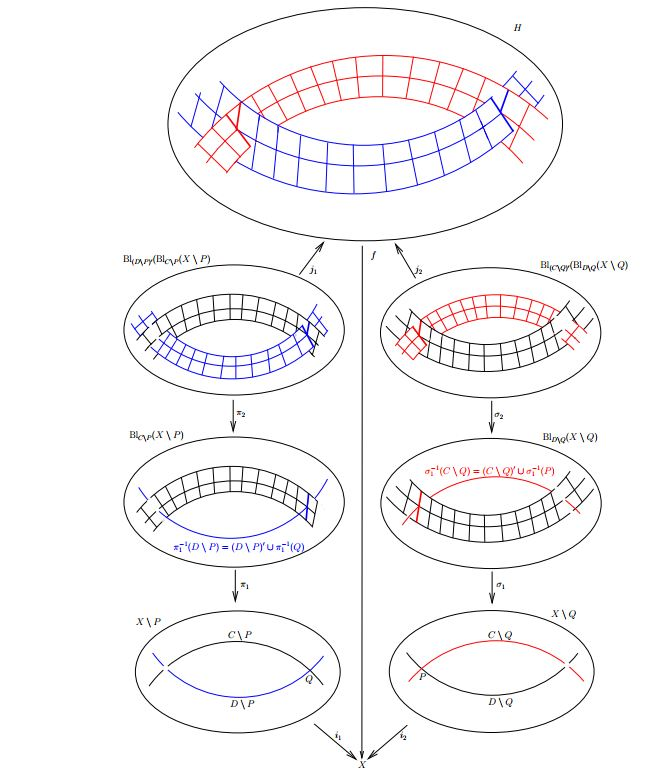
\includegraphics[width=\textwidth]{img/hironaka.JPG}
\caption{Hironaka’s example of a complete but non-projective variety; Ulrich Thiel}
\label{fig:Hironaka’s example}
\end{figure}
First we give the  construction of Hironaka's example. Let $X$ be a projective $3$-fold,  $C,D$ be two curves in $X$ intersecting at two points $P,Q$ transversely. To be more precise, we can just consider  
$$X=\mathbb{P}_{k}^{3}=\mathrm{Proj}(k[x,y,z,w]),C=\mathrm{Proj}(k[x,y,z,w]/(xy-z^{2},w)),D=\mathrm{Proj}(k[x,y,z,w]/(xy-w^{2},z)),$$
$$P=[1,0,0,0], Q=[0,1,0,0].$$
We have a $\mathbb{Z}/2\mathbb{Z}=\{1,g\}$-action on $X$ which switches $C,D$ and $P,Q$.   
$$g([x,y,z,w])=[y,x,z,w].$$
The construction is clear in the figure above(blow-up two open subscheme in different orders).  Let $\pi=\pi_{2}\circ \pi_{1} , \sigma=\sigma_{2}\circ \sigma_{1}$. On $U=X\setminus\{P,Q\}$, the order of the blow-ups doesn't matter, so we can glue the two blow-ups along $\pi^{-1}(U)\cong \sigma^{-1}(U)$. Then we get a variety $H$. Let's do some local computations to find out the exceptional divisors. Locally, 
\begin{itemize}
\item The first blow-up looks like $Bl_{(x,y)}\mathbb{A}_{k}^{3}$, which is just the closed variety in $\mathbb{A}_{k}^{3}\times \mathbb{P}_{k}^{1}$ defined by $xv-yv=0$. The local picture of the exceptional divisor is a hypersurface given by  $\mathrm{Proj}(k[x,y,z][u,v]/(xv-yu))\cong \mathbb{A}_{k}^{1}\times \mathbb{P}_{k}^{1}$.
\item The total transformation of $D$. Consider two affine charts of $Bl_{C}X$, $U_{1}=D_{+}(u), U_{2}=D_{+}(V)$, then we can write down the local equations 
\begin{itemize}
\item $$Bl_{C}X\cap U_{1}\cap \pi_{1}^{-1}(D)=\{y=vx, y=0,z=0\}= \{x=y=z\}\cup \{y=z=v=0,x\neq 0\}\cong D',$$ where $D'$ is the strict transformation of $D$.
\item $$Bl_{C}X\cap U_{2}\cap \pi_{1}^{-1}(D)=\{yu=x, y=0,z=0\}= \{x=y=z\}=\pi^{-1}(Q)\cong \mathbb{P}_{k}^{1}:=M_{1}.$$
\end{itemize}
\item Note that all the blow-ups are smooth, thus the local picture of $\pi_{2}$(also $\sigma_{2}$), but give us a different line as a new exceptional divisor $M_{2}$ over $Q$. 
\item Denote the exceptional hypersurfaces of $\pi_{1},\pi_{2}, \sigma_{1},\sigma_{2}$ by $E_{1}, E_{2}, F_{1}, F_{2}$, then we can glue $E_{1}$ and $F_{2}$ which gives us the red surface $S_{1}$ , glue $E_{2}$ and $F_{1}$ gives us the blue surface $S_{2}$, in the figure above.
\item Let $f:H\rightarrow X$, then $f^{-1}(P)=\{L_{1}, L_{2}\}\subset S_{1}$, $f^{-1}(Q)=\{M_{1}, M_{2}\}\subset S_{2}.$ Denote $f_{1}=f|_{S_{1}}, f_{2}=f|_{S_{2}}.$


\end{itemize}

Now we can prove $H$ is not projective nut complete. 
\begin{itemize}
\item For projectivity, since $C,D$ are just plane quadrics, they're isomorphic to $\mathbb{P}_{k}^{1}$(not to say rational). Consider $A\in C\setminus\{P,Q\}, B\in D\setminus\{P,Q\}$, by pulling back to $S:=S_{1}\cup S_{2}$(the union of the red and the blue surface), we get 
$$A\sim_{C} Q\Rightarrow f_{1}^{-1}(A)\sim_{S_{1}} M_{1}+M_{2},$$
$$B\sim_{D} P\Rightarrow f_{2}^{-1}(B)\sim_{S_{2}} L_{1}+L_{2}.$$
Similarly,
$$A\sim_{C} P\Rightarrow f_{1}^{-1}(A)\sim_{S_{1}} L_{2},$$
$$B\sim_{D} Q\Rightarrow f_{2}^{-1}(B)\sim_{S_{2}} M_{2}.$$
Now consider these relations in $S$, we get 
$$L_{1}+M_{1}\sim_{S} 0.$$
We get an effective algebraic cycle equivalent to $0$! This is impossible for a projective variety. We conclude that $H$ is not projective.
\item For completeness, we only need to prove that $\alpha: H\times Y\rightarrow Y$ is closed for any variety $Y$. Let $\beta X\times Y\rightarrow Y$ be the projection, then we have $\alpha=\beta\circ (f\times id).$ $\beta$ is a closed morphism since $X$ is projective. When restricted to $U_{1}(f\times id)^{-1}(X\setminus P), U_{2}=(f\times id)^{-1}(X\setminus Q)$, $f\times id$ is just a composition of blow-ups, locally, this gives us an isomorphism or the projection $\mathbb{A}_{k}^{3}\times \mathbb{P}_{k}^{1}\rightarrow \mathbb{A}_{k}^{3}$, which is closed. In short, $f\times id$ is closed and $H$ is universally closed, $H$ is compelte. 
\end{itemize}








\end{example}

\begin{remark}
Note that $$\mathrm{Proj}(k[x,y,z,u,v]/(xv-yu))\not\simeq\mathrm{Proj}(k[x,y,z]\oplus (x,y)\oplus(x,y)^{2}\oplus \dots ).$$
But we do have 
$$k[x,y,z]\oplus (x,y)\oplus(x,y)^{2}\oplus \dots \cong \mathrm{Proj}(k[x,y,z][u,v]/(xv-yu)).$$
Consider the natural map 
$$\mathrm{Proj}(k[x,y,z][u,v]/(xv-yu))\rightarrow \mathrm{Proj}(k[u,v]),$$
the fibre over $(v)$ is given by $\mathrm{Proj}(k[x,y,z][u]/(yu))$, but this is the same as $\mathrm{Spec}(k[x,y,z])$ since if a relevant homogeneous prime ideal contains $yu$, it must contains $y$. However, this remark is kind of redundant since the geometry is quite clear: the normal bundle $N_{C}X|_{C}\cong \mathcal{O}(1)^{2}$, or it just means planes passing $L=(x,y)$ are parametrized by $\mathbb{P}^{1}.$ 
\end{remark}
\begin{remark}
This construction could be simplified by considering two curves intersecting transversely at only one point. Then we should get something like $L_{1}+L_{2}\sim M_{1}, M_{1}\sim L_{2}\Rightarrow L_{1}\sim 0.$
\end{remark}



\begin{example}[Hironaka's example, Moishezen manifold of dimension $3$ but not algebraic]

\end{example}
\begin{example}[Hironaka's example, a deformation of Kähler manifolds that is not a Kähler manifold]
First note that the obstruction comes from the fact that we can find an effective cycle on a special fibre $V_{0}$ is algebraically equivalent to $0$, hence holomorphically equivalent to $0$. Hence the integral of any closed $(1,1)$-form cannot give a positive definite hermitian metric. This implies $V_{0}$ isn't Kähler. 

The idea of Hironaka's construction is the same as above: gluing blow-ups on different open subvarieties. Let 
$$X=\mathrm{Proj}(k[x,y,z,w])=\mathbb{P}_{k}^{3},W_{0}=D_{+}(x), W_{1}=D_{+}(y).$$
$$I_{C_{1}}=(z,w), I_{C_{2}}=(xy+yz+zx,w), I_{C_{3,t}}=((y+w)(x+ty)+yw,z).$$
\begin{itemize}
\item $t=0$, these three curves are smooth with common point $p=[1,0,0,0], q=[0,1,0,0].$
\item $t\neq 0$, $C_{1}\cap C_{2}\cap C_{3,t}=p=[1,0,0,0], C_{1}\cap C_{3,t}=\{p,q_{t}=[-t,1 ,0,0]\}.$
\end{itemize}
Now we start constructing the two blow-ups, 
$$T:=\mathbb{A}_{k}^{1}, H=X\times T$$
$$F_{1}=C_{1}\times T, F_{2}=C_{2}\times T, F_{3}=C_{3,t},$$
$$P=p\times T, Q=q\times T,$$
$$U_{0}=W_{0}\times T=\mathrm{Spec}(k[z_{1},z_{2},z_{3},t]), U_{1}=W_{1}\times T=\mathrm{Spec}(k[y_{0},y_{2},y_{3},t]),$$
$$U'=W_{0}\cap D_{+}(x+ty)=\mathrm{Spec}(k[z_{1},z_{2},z_{3},t, (1+tz_{1})^{-1}]). P\subset U'.$$
We're going to work over $H=(H\setminus P)\cup U'$(they play the roles of $X-P$ and $X-Q$ in the example above respectively.) Let 
$$x_{1}(t)=(1+tz_{1})(z_{1}+z_{2}+z_{3}+z_{1}z_{2})+z_{1}z_{3}, x_{2}=z_{2}, x_{3}=z_{3}.$$
Then the prime ideals of $F_{1}, F_{2}, F_{3}$ in $U'$ are given by $(x_{2},x_{3}), (x_{3}, x_{1}(t)), (x_{1}(t), x_{2})$ respectively. We glue $Bl_{\cup_{i=1}^{3}C_{i}}(H\setminus P)$ and $Bl_{I(t)}(U')$ along $U'\cap H\setminus P,$ where 
$$I(t)=(x_{1}(t)x_{2},x_{2}x_{3}, x_{3}x_{1}(t))(x_{1}(t), x_{2}x_{3})(x_{2},x_{3}x_{1}(t))^{2}(x_{3},x_{1}(t)x_{2})^{2}.$$
Note that in $U'$ we have a primary decomposition
$$I(t)=(x_{2},x_{3})^{5}\cap(x_{3},x_{1}(t))^{4}\cap(x_{1}(t),x_{2})^{4}\cap(x_{1}(t), x_{2}, x_{3})^{7}.$$
From this we can prove the following 
\begin{itemize}
\item two blow-ups are isomorphic in the overlap.
\item the fibre $V_{0}$ is not projective, not a Kähler manifold.
\item $V_{0}$ is smooth.
\item all other fibres $V_{t}, t\neq 0$ are smooth projective variety, hence are all Kähler manifold.
\end{itemize}
To demonstrate, we prove $V_{0}$ is smooth over $p$, which means we have to prove the blow-up of $\mathbb{A}_{k}^{3}$ of the ideal $(x_{1}x_{2},x_{2}x_{3}, x_{3}x_{1})(x_{1}, x_{2}x_{3})(x_{2},x_{3}x_{1})^{2}(x_{3},x_{1}x_{2})^{2}$ is smooth. We first blow-up the ideal $I_{1}=(x_{1},x_{2},x_{3}, x_{3}x_{1})$ and then the rest three. This is just a local computation
$$X'=Bl_{I_{1}}(\mathbb{A}_{k}^{3})=\mathrm{Proj}(k[x_{1},x_{2}, x_{3}][a,b,c]/(x_{1}x_{2}b=x_{2}x_{3}a, x_{1}x_{2}c=x_{3}x_{1}a,x_{2}x_{3}c=x_{3}x_{1}b))\subset \mathbb{A}_{k}^{3}\times \mathbb{P}_{k}^{2}.$$
This is cyclic symmetric, we only need to consider $D_{+}(a)$, and let $[u,v]=[\frac{b}{a}, \frac{c}{a}]$, then this first-step blow-up is given by 
$$x_{3}=ux_{1}, x_{3}=vx_{2}, x_{2}v=x_{1}u\Rightarrow Bl_{I_{1}}(X)\cong \{x_{2}v=x_{1}u\}\subset \mathbb{A}_{k}^{4}.$$
The origin is the only singularity. Now $(x_{1}, x_{2}x_{3}), (x_{2},x_{1}x_{3})$ becomes principal ideals and so in the second step, we only need to blow-up the ideal $(x_{3}, x_{1}x_{2})=(x_{1})\cap (u,x_{2})$, that is, just blow-up the ideal $J=(u, x_{2}).$ Then $X''=Bl_{J}(X')$ is a closed subvariety in $X'\times \mathbb{P}_{k}^{1}$ given by the equations $u\beta=x_{2}\alpha.$ Then in $D_{+}(\alpha)$, let $z=\frac{\beta}{\alpha}$, $X''$ is given by
$$x_{1}=vz, x_{2}=vz, x_{3}=uvz.$$
This is smooth, isn't it? Hence, we're done. we also have a question 
$$\text{Is $H$ smooth, and why?}$$
\end{example}
\begin{remark}[Blow-ups]
Note the following 
\begin{itemize}
\item blow-up is not sensible to the non-reduced structures.
\item the blow-up of the ideal $I=(x_{1}x_{2},x_{3})^{4}\cap (x_{2},x_{3})$ is smooth, why we have to argue like `after the blow-up of the ideal $(x_{2},x_{3})$, the pull-back becomes a principal ideal or the ideal of a smooth curve, hence the blow-up of the $I$ is smooth?'
\end{itemize}
\end{remark}



\begin{remark}
Why some closed $(1,1)$-form on a Kähler manifold  should give me positive definite hermitian metric by integration against topological $2$-cycles? 
\end{remark}
\begin{remark}[why this construction doesn't work with two curves?]
This is a typical phenomenon in algebraic geometry: we can define a family of curves(e.g. quadrics) $X_{t}$ over some base, although topologically, every fibre is quite clear, however, you might get some non-reduced fibres, this makes it hard to talk about concepts like complex structure, Kähler metric, because the correspondence provided by GAGA doesn't exist anymore. For example, consider a family of skew lines in $\mathbb{A}_{k}^{3}$ parametrized by $\mathbb{A}_{k}^{1}:$
$$X_{t}=\mathrm{Spec}(k[x,y,z][t]/(x,y)\cap (x-t,z))=\mathrm{Spec}(k[x,y,z][t]/(yz,xz,xy-yt,x^{2}-xt)).$$
Then it's obvious $\mathcal{O}_{X_{0}}=k[x,y,z]/(yz,xz,xy,x^{2})$ is not reduced!
\begin{figure}[h!]
\centering
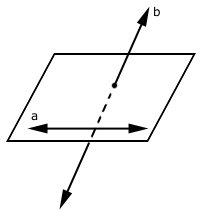
\includegraphics[width=0.3\textwidth]{img/skewlines.jpg}
\caption{Family of skew lines, non-reduced limit}
\label{fig:Family of skew lines, non-reduced limit}
\end{figure}
\end{remark}
\begin{remark}[symplectic manifold, non-Kähler]
First recall that one of the obstructions comes from the existence of the Hodge decomposition on a Kähler manifold. Kodaira-Thurston's example below is a symplectic $4$-manifold with odd first Betti number, thus non-Kähler. i.e.
$$X=(T^{3}\times \mathbb{R})/\mathbb{Z}, n\bullet(x,y,z,t)=(x,y+nx, z, t+n).$$
$$\omega_{X}=dx\wedge dy+dz\wedge dt.$$
We can view $X$ as a symplectic torus fibration over the $(z,t)$-torus or as a Lagrangian torus fibration over the $(x,z)$-torus. Let's use the first fibration. The natural map $\pi: \mathbb{R}^{4}\rightarrow X$ is the universal covering of $X$, the Deck transformation can be read from 
$$(x,y,z,t)\mapsto (x+a, y+b+d(x+a), z+c, t+d).$$
i.e we can view it as a (non-commutative) group structure $\Gamma$ defined on the set $\mathbb{Z}^{4}$,
$$(a,b,c,d)\star (a',b',c',d')=(a+a', b'-d'a, c+c', d+d').$$
Thus $\mathrm{rank}([\Gamma, \Gamma])=1$, the commutator subgroup is generated by $(0,1,0,0)$, it gives us the abelianization 
$$H_{1}(X,\mathbb{Z})\cong \Gamma/[\Gamma,\Gamma]\cong \mathbb{Z}^{3}.$$
This cannot be a Kähler manifold. McDuff also has an example based on Kodaira-Thurston's. For details, see 
\href{http://www.homepages.ucl.ac.uk/~ucahjde/ST-lectures/lecture11.pdf}{this notes}
\end{remark}


\subsection{Alterations}
\begin{example}[Reduced scheme, after base-change nowhere reduced, Macaulay]
Let $k=\mathbb{F}_{p}(u,v)$, 
$$C:=\mathrm{Spec}(A)=\mathrm{Spec}(k[x,y]/(ux^{p}+vy^{p}-1))\subset \mathbb{A}_{k}^{2}.$$
Then 
\begin{itemize}
    \item $A$ is Dedekind
    \item $k\subset \mathrm{Frac}(A)$ is relatively algebraically closed
    \item $k'=\mathbb{F}_{p}(u^{\frac{1}{p}}, v^{\frac{1}{p}})$, then $C\times_{k'}k$ is nowhere reduced.
\end{itemize}
\end{example}
\begin{example}[Strict normal crossing divisor]

\end{example}
\begin{example}[A non catenary Noetherian local ring, Stacks project, Tag 02JE]
\href{http://stacks.math.columbia.edu/tag/02JE}{Here}
\end{example}
\begin{remark}[Cohen-Macaulay rings, Dedekind domains, Complete local noetherian rings , Regular rings]
\end{remark}

\begin{example}[A discrete valuation ring but not a $G$-ring]
\href{http://download.springer.com/static/pdf/44/bok%253A978-3-642-51438-8.pdf?originUrl=http%3A%2F%2Flink.springer.com%2Fbook%2F10.1007%2F978-3-642-51438-8&token2=exp=1496253532~acl=%2Fstatic%2Fpdf%2F44%2Fbok%25253A978-3-642-51438-8.pdf%3ForiginUrl%3Dhttp%253A%252F%252Flink.springer.com%252Fbook%252F10.1007%252F978-3-642-51438-8*~hmac=50e8488a6e07258b7a5a4a5db610c4d244c0166f45a353e06d08637f96b5c0ca}{BLR, Neron model,page82, example 11}. And in Qing Liu's book, Example $8.2.31$
\end{example}



















\begin{example}[Akizuki's example, a noetherian local integral domain whose normalization is not finite]
Let 
\begin{itemize}
\item $A$, a $\mathrm{DVR}$
\item $t$, the local parameter
\item $k=A/(t)$, the residue field
\item $\hat{A}$, the completion of $A$ w.r.t $(t)$
\item assume $\hat{A}$ has a transcendental element over $A$
\end{itemize}
For example, we can take
\begin{itemize}
\item $A=\mathbb{Z}_{(p)}$, the localization of $\mathbb{Z}$ at the prime ideal $(p)$
\item $t=p$, the local parameter
\item $k=\mathbb{F}_{p}$
\item $\hat{A}=\mathbb{Z}_{p}$, the ring of $p$-adic integers
\end{itemize}
or
\begin{itemize}
\item $A=k[t]_{(t)}$, the localization of $k[t]$ at the prime ideal $(t)$
\item $t$, the local parameter
\item $k$, the residue field
\item $\hat{A}=k\llbracket t\rrbracket$, the ring of formal power series
\end{itemize}
We first give the construction of Akizuki's example,
\begin{itemize}
\item $z=z_{0}=a_{0}+a_{1}t^{n_{1}}+\dots + a_{k}t^{n_{k}}+\dots \in \hat{A}$ such that 
\begin{itemize}
\item $a_{i}\in A^{\times}$
\item $n_{i+1}>2n_{i}+2$
\item $z$ is transcendental over $A$, thus $A[z]\subset \hat{A}$ is just the polynomial ring of one variable over $A$
\item $A=\mathbb{Z}_{(p)}$, we may take $z=\sum\frac{1}{(p+1)^{n}}p^{n!}$. $A=k[t]$, we may take $z=\sum t^{n!}$
\end{itemize}

\item $z_{r}=\frac{z_{0}-\text{first $r$ terms}}{t^{n_{r}}}=a_{r}+a_{r+1}t^{n_{r+1}-n_{r}}+\dots$. Let $m_{r}=n_{r}-n_{r-1}$, we have $m_{r}>n_{r-1}+2$.
\item $z_{r}-a_{r}=t^{m_{r+1}}z_{r+1}$
\item $t^{n_{r}}z_{r}=z_{0}-\sum_{i=0}^{r-1}a_{i}t^{n_{i}}$
\item $$B=A[z_{0}, z_{1},\dots ]=A[(z_{0}-a_{0}), (z_{1}-a_{1})\dots ]$$
$$B_{m}=A[z_{0},a_{1},\dots ]_{(t)}$$
$$C=A[t(z_{0}-a_{0}), \{(z_{i}-a_{i})^{2}\}_{i=1}^{\infty}]$$
$$C_{M}=A[t(z_{0}-a_{0}), \{(z_{i}-a_{i})^{2}\}_{i=1}^{\infty}]_{(t)}$$
\item The final claim is that 
$$\text{$C_{M}$ is a $1$-dimensional integral noetherian local ring} $$
$$\text{$B_{m}$ is the normalization of $C_{M}$ in $\mathrm{Frac}(C_{M})=\mathrm{Frac}(B_{m})=A(z)$}$$
$$\text{$B_{m}$ is not finite over $C_{M}$}$$
\end{itemize}
Now let's give the proof. The main observation is that 
$$\text{$0\neq f\in M$, the principal ideal $fC_{M}\subset C_{M}$ contains some power of $t$}$$
First, we should ask, what an element  $f\in C$ looks like? Well, it's a polynomial in $t(z_{0}-a_{0}), (z_{i}-a_{i})^{2}$, topologically, we want to describe $f$ as a point in some small neighborhood of a point in $A$. How to do this? Just by raising the power of $t$. It's not hard because we can 
\begin{itemize}
\item  we can always replace $t(z_{0}-a_{0})$ by $t^{n_{i}+1}(z_{i}-a_{i})$, the difference lies in $A$. Replacing $t^{n_{i}+1}(z_{i}-a_{i})$ by $t^{n_{j}+1}(z_{j}-a_{j})$ if we want to raising the power of $t$ further. 
\item we can replace $(z_{i-1}-a_{i-1})^{2}$ by $t^{2m_{i}}(z_{i}-a_{i})^{2}+\text{multiple of } t^{n_{i}+2}(z_{i}-a_{i})+\text{somthing in $A$}$. This is because (remember $m_{i}>n_{i}+2$)
$$(z_{i-1}-a_{i-1})^{2}=(t^{m_{i}}z_{i})^{2}=t^{2m_{i}}((z_{i}-a_{i})^{2}-a_{i}^{2})+2a_{i}t^{2m_{i}}z_{i}$$
\item That is, any $f\in C, r, N$ positive integers, we can write it as 
$$f=\alpha+\beta t^{n_{r}+1}(z_{r}-a_{r})+t^{N}\theta, \alpha,\beta\in A, \theta\in C.$$
\item $0\neq f\in M$, thus exists $N>0$ such that $f\notin t^{N}\hat{A}$, we may choose $r$ such that $n_{r}+1>N$. Then we know $\alpha=t^{k}u$, and $k<N, u\in A^{\times}$. Dividing both sides by $u$, we may assume 
$$f=t^{k}(1+t^{N-k}\theta)+\beta t^{n_{r}+1}(z_{r}-a_{r})$$
Let $$g=t^{k}(1+t^{N-k}\theta)-\beta t^{n_{r}+1}(z_{r}-a_{r})$$
We have 
$$fg=t^{2k}(1+t^{N-k}\theta)^{2}-\beta t^{2n_{r}+2}(z_{r}-a_{r})^{2}=t^{2k}v, v\in C\setminus M$$
Then we know $t^{2k}\in fC_{M}$.
\item It follows that any proper prime ideal in $C_{M}$ contains $t$, thus $\mathrm{Spec}(C_{M})=\{0, C_{M}\}$, in other words, it's a $1$-dimensional local ring.
\item To see $C_{M}$ is noetherian, first notice that $C_{M}/(t^{N}C_{M})$ is a finite $A/(t^{N})$-module generated by $\{1,t^{n_{r}+1}z_{r+1}\}$. Now any nonzero ideal $I\subset C_{M}$, we know $(t^{N})\subset I$, thus $C_{M}/I$ is a quotient of $C_{M}/(t^{N}C_{M})$ as an $A$-module, thus Noetherian. 
\item Now it's clear that $C_{M}$ is an integral, noetherian local ring of dimension $1$.
\item We only need to prove that $B_{m}$ is not finite over $C_{M}$. Just consider the ascending chain of submodules generated by $\{z_{i}-a_{i}\}_{i=1}^{r}$, if it's stable, then we must have 
$$z_{r}-a_{r}=\sum_{i=1}^{r-1} \theta_{i}(z_{i}-a_{i}), \theta_{i}\in C_{M}.$$
We may assume $\theta_{i}=\frac{\alpha_{i}}{\gamma}$, wher $\alpha_{i}\in C, \gamma\notin M$, we get 
$$\gamma(z_{r}-a_{r})=\sum_{i=1}^{r-1} \alpha_{i}(z_{i}-a_{i}).$$
Multiplying both sides by $t^{n_{r}}$, we get an algebraic equation w.r.t $z$
$$\gamma(z-\sum_{i=0}^{r+1}a_{i}t^{n_{i}})=\sum_{i=1}^{r-1} \alpha_{i}t^{n_{r}-n_{i}}(z-\sum_{j=0}^{j+1}a_{j}t^{n_{j}})$$
Note that $\gamma$ is a unit in $C_{M}$, coefficients on the right hand side are all divided by some positive power of $t$, every $\alpha_{i}$ is a polynomial in $z$ over $A$. Thus this equation is an non-trivial polynomial, whcih contradicts the fact that $z$ is transcendental over $A$. Now everything is clear.
\end{itemize}

More details and discussion of Akizuki's example can be found in \href{https://arxiv.org/pdf/alg-geom/9503017.pdf}{Akizuki's counterexample}
\end{example}
\begin{remark}
For integral schemes of finite type, the normalization is always finite. My personal feeling is that, to consider geometric questions, we have to assume a scheme is of finite type over $k$ or $\mathbb{Z}$ at some point.
\end{remark}
\begin{remark}
\href{https://math.stackexchange.com/questions/879962/does-it-hold-that-the-p-adic-completion-of-the-integers-equals-the-completion}{p-adic completion of the integers equals the completion}
\end{remark}


\begin{example}[a flat and finite type morphism between noetherian schemes, fibres have different dimensions]
Let $R$ be your favorite DVR (for example, $\mathbb{Z}_{(p)}, k[t]_{(t)}$). Our palyers are 
\begin{itemize}
\item $Y=\mathrm{Spec}(R)$, $(0)$ is the generic point, which is open in $Y$ with residue field $K=\mathrm{Frac}(R)$, $\mathfrak{m}$ is the unique maximal ideal, which is closed in $Y$ with residue field $k=R/\mathfrak{m}$.
\item Glue $\mathbb{A}_{R}^{1}=\mathrm{Spec}(R[x])$ along $(\mathbb{G}_{m})_{K}\subset \mathbb{A}_{R}^{1}$ with a union of $\mathbb{A}_{K}^{1}$ and $\mathbb{P}_{K}^{2}$ meeting at the origin by inversion. That is, at the generic fibre, we get a union of $\mathbb{P}_{K}^{1}$ and $\mathbb{P}_{K}^{2}$. Denote the glued scheme by $X$. 
\item $\pi:X\rightarrow Y$ gives us a flat morphism since all modifications happen at the generic fibre. 
\item $\pi$ is not proper because $\mathbb{P}_{K}^{2}$ is a closed subset of $X$, but the image of it is the genric point which is not closed. 
\item $\mathrm{dim}(Y_{(0)})=2$(not pure), $\mathrm{dim}(Y_{\mathfrak{m}})=1$. 
\href{https://mathoverflow.net/questions/7469/is-relatively-algebraically-closed-stable-under-finite-field-extensions}{.....}
\end{itemize}



\end{example}
\begin{remark}
In fact, we have 
\begin{itemize}
\item Let $f:X\rightarrow Y$ be a proper flat and finitely presented morphism(no assumption on irreducibility, noetherian hypothesis), $y\mapsto \mathrm{dim}X_{y}$ is a locally constant function.
\item Let $f:X\rightarrow Y$ be a flat and finite type morphism between noetherian schemes, $d:=\mathrm{dim}X_{\eta_{Y}}$, then all geometric fibres $X_{\bar{y}}$ has pure dimension $d$.
\end{itemize}


\end{remark}








































\begin{example}[non-Gorenstein variety]
\href{https://arxiv.org/pdf/math/0209199.pdf}{Hyman Bass and Ubiquity: Gorenstein Rings}
\end{example}

\begin{example}[valuation rings and discrete valuation rings]

\end{example}

\begin{example}[Brian Conrad's notes, page69, a semi-stable curve over a noetherian scheme with smooth generic fibre is normal]

\end{example}

\begin{example}[smooth morphism, isomorphic generic fibre, nonisomorphic special fibres, Shizhang]
Let $V=\mathcal{O}\oplus\mathcal{O}(2), W=\mathcal{O}\oplus\mathcal{O}$ over $\mathbb{P}^{1}_{k\llbracket t\rrbracket}$
$$\begin{tikzcd} \mathbb{P}(V)\arrow{rd}{f} & & \mathbb{P}(W)\arrow{dl}{g} \\
&\mathrm{Spec}(k\llbracket t\rrbracket) &\end{tikzcd}$$
\end{example}
\begin{remark}[no fine Moduli space for semi-stable vector bundles]
First note that this example can be extended to all $F_{n}$ surfaces. 
\end{remark}
\begin{example}[smooth varieties over a DVR, isomorphic generic fibres, nonisomorphic special fibres]
\href{https://mathoverflow.net/questions/75393/does-isomorphic-generic-fibre-imply-isomorphic-special-fibre-for-smooth-morphism}{Here}
\end{example}
\begin{example}[resolution of singularities of semistable curves over a discrete valuation ring]
Let $R$ be a discrete valuation ring(e.g $k\llbracket t\rrbracket$), $\pi$ a uniformizer and $n\geq 1$, consider 
$$C_{n}:\mathrm{Spec}R[x,y]/(xy-\pi^{n}).$$
Then the generic fibre is smooth($\pi$ is invertible in $\mathrm{Frac}(R)$), its special fibre is singular at a unique point $p=(x,y)$, the completion is given by 
$$\widehat{\mathscr{O}_{C_{n},p}}=\widehat{R}[x,y]/(xy-\pi^{n})$$

Brian Conrad's notes on alteration page78.
\end{example}
\begin{example}[Henselization]
\href{http://stacks.math.columbia.edu/tag/03QD}{Stacks project Tag 03QD}
\href{https://en.wikipedia.org/wiki/Henselian_ring}{Wikipedia Henselian rings} and example of \href{https://math.stackexchange.com/questions/2143409/algebraic-formal-power-series}{algebraic formal power series}
\end{example}

\begin{example}[page 11, imperfect field geometrically integral curve , $k(x)/k$ not separable]

\end{example}




\begin{example}[Complete local rings]
Complete local rings are not hard to get. Just take any local ring and compute the completion. For example
\begin{itemize}
\item $R=k\llbracket x, y\rrbracket/(xy)$ is the completion of the local ring at the node of the nodal curve $y^{2}=x^{2}(x+1)$. It's not regular. Since the minimal number of generators of $\mathfrak{m}=(x,y)$ is 2. But the Krull dimension is just $1$. To see this any prime $\mathfrak{p}$ is generated by some $x^{n}u$ and $y^{m}v$ where $u, v$ are invertible elements in this complete ring.
For the ideal to be a prime, the only possibility is that $n=m=0$. Notice that $(0)$ is not a prime ideal of this ring. We get $\mathrm{dim}R=1$.
\item $R= \mathbb{Z}_p\llbracket x,y\rrbracket/(xy-v)$ is the completion of $\mathbb{Z}_p[x,y]/((x^2-2+y^2)(x^2-y^2)+p^ry)$. 
\end{itemize}
\end{example}

\begin{example}[A regular local ring does not contain a field]
The localization of $\mathbb{Z}[X]$ at the maximal ideal $(2,x)$, that is $\mathbb{Z}[x]_{(2,x)}$ is a dimension $2$ regular local ring which does not contain any field.
\end{example}

\subsection{Smoothness and regularity}
\begin{example}[Varieties singular everywhere]
If $X$ is a variety over an algebraically closed field $k$ and $char(k)=0$, we know we can find an open subset $U\subset X$, such that $U$ is smooth. This is not true for prime characteristics, consider $\overline{\mathbb{F}}_{p}$
$$V: x_{0}^{p}+x_{1}^{p}+\dots + x_{n}^{p}$$
is singular everywhere, I know this example is silly, but it's an example...
\end{example}







\begin{example}[Morphism singular everywhere]
Let $k=\overline{\mathbb{F}}_{p}$, consider the Frobenius morphism
$$f:X=\mathbb{P}_{k}^{n}\rightarrow \mathbb{P}_{k}^{n}=Y$$
$$[x_{0},\dots, x_{n}]\mapsto [x_{0}^{p},\dots, x_{n}^{p}].$$
Note that we have the conormal sequence 
$$f^{*}\Omega_{Y/k}\rightarrow \Omega_{X/k}\rightarrow \Omega_{X/Y}\rightarrow 0$$
Since $d(x_{i}^{p})=0$, the first map in the sequence is $0$, $\Omega_{X/Y}\cong \Omega_{X/k}$ is locally free of rank $1\neq 0=\mathrm{dim}(X)-\mathrm{dim}(Y).$ Or it's natural to see the induced map on tangent space is not surjective(it's $0$)

\end{example}





\begin{remark}[Normal, conormal, tangent, cotangent, canonical]
\end{remark}



\begin{example}[Nonperfect field, regular $\neq$ smooth]
Let $k=\mathbb{F}_{p}(t), p>2$, consider 
$$C:y^{2}=x^{p}-t \subset \mathbb{A}_{k}^{2}.$$
Then every local ring of $C$ is regular but $C$ is not smooth over $k$. First the Jacobian matrix is given by
$$(2y, 0)$$
So it only vanishes at the prime ideal $\mathfrak=(y, x^{p}-t)$. So we only need to prove
\begin{itemize}
\item the regularity of 
$$\mathcal{O}_{C,\mathfrak{p}}=(k[x,y]/(y^{2}-x^{p}+t))_{(y,x^{p}-t)}$$
\item $C$ is not smooth after some base change.
\end{itemize}
The first statement is because $\mathcal{O}_{C,\mathfrak{p}}$ is domain and a local ring with dimension $1$, its maximal ideal is generated by $y$, thus $\mathcal{O}_{C,\mathfrak{p}}$ is a DVR, hence regular. Then we base change it to $K=\mathbb{F}_{p}(t^{\frac{1}{p}})$. Then we get 
$$C_{K}: y^{2}=(x-t^{\frac{1}{p}})^{p}$$
Then it's not smooth at $\mathfrak{q}=(y,x-t^{\frac{1}{p}})$, it's not even normal, consider 
$$\alpha=\frac{y}{x-t^{\frac{1}{p}}}\in Frac(\mathcal{O}_{C_{K}, \mathfrak{q}})$$
Then $$\alpha^{2}=\frac{y^{2}}{(x-t^{\frac{1}{p}})^{2}}=(x-t^{\frac{1}{p}})^{p-2}\in \mathcal{O}_{C_{K},\frak{q}}.$$
Note that the Auslander–Buchsbaum theorem states that every regular local ring is a unique factorization domain, hence normal. $\mathcal{O}_{C_{K},\mathfrak{q}}$ is not normal, not to say regular.
\end{example}



\begin{remark}[Jacobian criterion]
$$dim_{k(x)}(\Omega_{X/k}\otimes k)=n-\mathrm{rank}J_{x}$$
my question is what is $J_{x}$ at a nonclosed point $x$? Actually you always compute the ordinary Jacobian, but to determine its rank, you have to ask at what point? See $x$ corresponding to a prime ideal $\mathfrak{p}$, and $$C:=\mathrm{Spec}(k[x_{0},x_{1},\dots, x_{n}]/(f_{1},\dots, f_{m}))$$
Let $\Dealta_{m}$ be a $m\times m$ minor of the Jacobian matrix, to determine it's smooth or not at $\mathfrak{p}$, you only need to check if $\Delta_{m}\in \mathfrak{p}$ or not. In general 
$$Jacobian \Rightarrow smooth \Rightarrow regular$$
\end{remark}



\begin{remark}[Different definitions of smoothness]
\end{remark}

\begin{example}[Regular $k$-algebra of dimension $1$, but not regular after base change to $\overline{k}$]
$$\mathcal{O}_{C,\mathfrak{p}}, \mathcal{O}_{C_{K},q}$$
above.
\end{example}


\begin{example}[Bertini theorem in characteristic $p$]
Consider the Frobenius map again
$$f:\mathbb{P}_{k}^{1}\rightarrow \mathbb{P}_{k}^{1}; [x,y]\mapsto [x^{p},y^{p}]$$
Then we know it's corresponding to the $1$-dimensional linear system $\mathfrak{d}=\{pP|P\in\mathbb{P}_{k}^{1}\}$, or in other words $\{(ax+by)^{p}|a,b\in k\}$, they're all singular. However Poonen proves a Bertini theorem for quasi-projective varieties over finite fields.
\end{example}





\begin{example}[A normal variety but not smooth, based on Hartshorne $\mathrm{II}.6.4$ ]
Just consider the cone $X$ in $\mathbb{A}_{k}^{3}$, assume that $char(k)\neq 2$
$$X: x_{0}^{2}=x_{1}^{2}+x_{2}^{2}$$
$X$ is singular at the vertex $(0,0,0)$. To see it's normal, we prove 
\begin{itemize}
\item Let $f \in k[x_1,\ldots,x_n]$ be a square-free nonconstant polynomial over a field of characteristic $\ne 2$. Then, $k[x_1,\ldots,x_n,z]/(z^2-f)$ is integrally closed.
\end{itemize}
Observe that $$K=\mathrm{Frac}(k[x_{1},\dots, x_{n}]/(z^{2}-f))=k(x_{1},\dots, x_{n})[z]/(z^{2}-f)$$ It's a Galois extension of degree $2$ over $k(x_{1},\dots, x_{n}) $. If $\alpha = g + hz \in K$, where $g,h \in k(x_1,\ldots,x_n)$. We know the minimal polynomial of $\alpha$ is
$\alpha^2 - 2g\alpha + (g^2-h^2f)$, because
  $$
    (g+hz)^2 - 2g(g+hz) + (g^2 - h^2f) = g^2 + 2ghz + h^2z^2 - 2g^2 - 2ghz + g^2 - h^2f = 0.
  $$
  Thus, $\alpha$ is integral over $k[x_1,\ldots,x_n]$ if and only if
  $2g$ and $g^2-h^2f \in k[x_1,\ldots,x_n]$, which is true if and only if $g, h^2f \in
  k[x_1,\ldots,x_n]$. Now if $\alpha$ is integral, and $h$ had nontrivial
  denominator, then $h^2 \notin k[x_1,\ldots,x_n]$ since $f$ is square-free;
  hence $h \in k[x_1,\ldots,x_n]$ so $\alpha \in k[x_{1},\dots, x_{n}]/(z^{2}-f)$. Thus, $k[x_{1},\dots, x_{n}]$ is integrally closed in $K$. As a special case we $k[x_{0},x_{1},x_{2}]/(x_{0}^{2}-x_{1}^{2}-x_{2}^{2})$ is normal and it's easy to check all its local rings are normal.
\end{example}

\begin{example}[A formally smooth morphism but not smooth]
 Consider the ring homomorphims $$p: k[t^{q}, q\in \mathbb{Q}_{>0}]\rightarrow k$$
 $$t^{q}\mapsto 0.$$
 It's not smooth simply because it's not flat. 
 $$0\rightarrow (t)\rightarrow k[t^{q}, q\in \mathbb{Q}_{>0}]\rightarrow k[t^{q}, q\in \mathbb{Q}_{(0,1)}]\rightarrow 0.$$ 
 After tensoring with $k$, the left hand side is not injective anymore. To prove it's formally smooth, let $A$ be a ring with a square zero ideal $I$, consider the following diagram,
 $$
 \begin{tikzcd}
 A/I & k \arrow{l}{g}\\
 A\arrow{u}{\pi} &  k[t^{q}, q\in \mathbb{Q}_{>0}]\arrow{l}{f}\arrow{u}[swap]{p}.
 \end{tikzcd}
 $$
 Then $f(t^{q})\in I$ since the diagram is commutative. However, every $t^{q}$ is a square, we thus have $f(t^{q})=f((t^{\frac{q}{2}})^{2})\in I^{2}=0$. In other words, $f$ factors through $p$, this is exactly the formal smoothness of the map $p$.
 
\end{example}



\end{document}
